\documentclass[%
  aspectratio=169,
  9pt,
%   t,
%  USenglish,
ngerman,
%   dark,
  light,
  mathserif,
%   serif, 
  professionalfont,
%  handout,
%  affiliationinhead,
  affiliationintitlepagehead,
  titlegraphic,
  %% The following options would violate the CD rules!
   affiliation,
%   uselogos,
   navigationbar,
  progressbar,
%   seprules,
%   titleinhead,
]{beamer}

\usepackage[utf8]{inputenc}
\usepackage[english, ngerman]{babel}
\usepackage[]{csquotes}

\usepackage{siunitx}

\sisetup{%
	mode = math,
	detect-family,
	detect-weight,  
	exponent-product = \cdot,
	number-unit-separator=\text{\,},
	output-decimal-marker={\text{,}},
	math-rm=\mathsf,
	text-rm=\sffamily,
}

\usepackage{animate}
%\usepackage{MnSymbol,wasysym}

%\newcommand{\org}{LMF}
% \newcommand{\org}{FPF}
%\newcommand{\coorg}{DLR}
\newcommand{\boldstruct}[1]{\textbf{\structure{#1}}}
\usetheme{TUM}
\usepackage{glossaries}
\usepackage{graphicx}
\usepackage{nth}
%\usepackage{natbib}
\usepackage[square,sort,comma,numbers]{natbib}
\bibliographystyle{abbrvnat}
\setcitestyle{authoryear}%,open={((},close={))}

\usepackage{tummath}
\usepackage{tumtensors} % experimental
\usepackage{tumcolors}
\usepackage{subfigure}
\usepackage[noabbrev, capitalize]{cleveref}
\usepackage{csvsimple}
\usepackage{colortbl}
\usepackage{tabularx}
\usepackage{multimedia}

\PassOptionsToPackage{cmyk}{xcolors}
	
\usepackage{booktabs}
\usepackage{contour}

%\usepackage{biblatex}
%\addbibresource{bib/ijgi}

\usepackage{pgfplots}
\usepgfplotslibrary{groupplots}
\usepackage{pgfplotstable}
\usepgfplotslibrary{dateplot}

%\usepgfplotslibrary{external}
%\tikzexternalize

\usepackage{booktabs}
\usepackage{array}
\newcolumntype{x}{l}
\newcolumntype{X}{>{}l}
\newcolumntype{v}[1]{>{\raggedright\hspace{0pt}}p{#1}}
\newcolumntype{V}[1]{>{\scriptsize\raggedright\hspace{0pt}}p{#1}}


\definecolor{fusionremovedcolor}{HTML}{00CA43}
\definecolor{fusionaddedcolor}{HTML}{FF00F7}
\definecolor{overlapcolor}{HTML}{FAC843}

\usepgfplotslibrary{external}
%\tikzexternalize
\tikzsetexternalprefix{tikz/}

%\usetikzlibrary{mindmap}

%\usetikzlibrary{arrows} 
%\usetikzlibrary{backgrounds}
\usetikzlibrary{fit}
%\usetikzlibrary{shapes}
\usetikzlibrary{calc}
\usetikzlibrary{positioning}
\usetikzlibrary{matrix}
\usepackage[nodayofweek,level]{datetime}
%\usepackage{mwe}
%%
%
\usetikzlibrary{3d}
\tikzstyle{perspective3d}=[
x={(0.5cm,0.5cm)}, y={(1cm,0cm)}, z={(0cm,1cm)}]


\colorlet{traincolor}{tumbluelight}
\colorlet{validcolor}{tumbluedark}
\colorlet{evalcolor}{tumorange}

\colorlet{forwardcolor}{tumblue}
\colorlet{backwardcolor}{tumorange}

\colorlet{activationcolor}{tumblue}
\colorlet{gridcolor}{tumgraylight}
\colorlet{contextonecolor}{tumorange}
\colorlet{contexttwocolor}{tumorange!80}
\colorlet{contextthreecolor}{tumorange!60}
\colorlet{contextfourcolor}{tumorange!40}

% defaultvalue -> might be replaced later
\colorlet{tensorcolor}{forwardcolor}

\colorlet{classcolor}{tumivory}
\colorlet{encodercolor}{tumblue}
\colorlet{encodercolor}{tumred}

%\usepackage{media9}

% notation
\newcommand{\MWeight}{\ensuremath{\M{W}}}
\newcommand{\VBias}{\ensuremath{\V{b}}}
\newcommand{\VInput}{\DataVec}
\newcommand{\VHidden}{\ensuremath{\V{h}}}
\newcommand{\FActivation}{\ensuremath{\sigma}}
\newcommand{\VCellState}{\ensuremath{\V{c}}}
\newcommand{\VForgetGate}{\ensuremath{\V{f}}}
\newcommand{\VModulationGate}{\ensuremath{\V{j}}}
\newcommand{\VInputGate}{\ensuremath{\V{i}}}
\newcommand{\VOutputGate}{\ensuremath{\V{o}}}



\newcommand{\VResetGate}{\ensuremath{\V{r}}}
\newcommand{\VUpdateGate}{\ensuremath{\V{u}}}

%\newcommand{\concat}[2]{\VecDef{#1 \Vert #2}}
\newcommand{\concat}[2]{[#1\Vert#2]}

\newcommand{\Rin}[3]{\mathbb{R}^{[#1 \times #2 \times #3]}}
\newcommand{\Rinfloor}[3]{\mathbb{R}^{[#1]} \times \mathbb{R}^{[#2]} \times \mathbb{R}^{[#3]}}
\newcommand{\Rinfour}[4]{\mathbb{R}^{[#1 \times #2 \times #3 \times #4]}}

% kernel size of rnn convolution
\newcommand{\krnn}{k_{rnn}}
% kernel size of classification convolution
\newcommand{\kclass}{k_{class}}

\newcommand{\eg}{e.g., }
\newcommand{\ie}{i.e. }

%\newcommand{\classname}[1]{\texttt{#1}}
\newcommand{\classname}[1]{\textsl{#1}} % what about \textsl for classnames?
\newcommand{\cn}[1]{\classname{#1}} % short alias

\newcommand{\nutzungscn}[1]{\textsc{#1}} % stmelf Nutzungsklassen

\newcommand{\brand}[1]{\textsc{#1}}
\newcommand{\processing}[1]{\brand{#1}}
\newcommand{\satellite}[1]{\brand{#1}}
\newcommand{\band}[1]{\brand{#1}}

% https://tex.stackexchange.com/questions/167925/how-to-make-maths-equations-start-at-the-left
\newcommand{\mathleft}{\@fleqntrue\@mathmargin0pt}
\newcommand{\mathcenter}{\@fleqnfalse}

\usetikzlibrary{spy}

% \usepackage[ngerman]{babel} % if you get errors on compile: rm *aux *out *log *nav *snm *toc

\newcommand{\rastergrid}{
	\input{images/rastergrid.tikz}
}
\newcommand{\vectorgrid}{
	\input{images/vectorgrid.tikz}
}

%\setbeamersize{description width=0mm}

\mode<handout>{
  \usepackage{pgfpages}
% feel free to use one of these layouts
%   \pgfpagesuselayout{1 on 1}[a4paper,border shrink=5mm]
  \pgfpagesuselayout{2 on 1}[a4paper,border shrink=5mm]
%   \pgfpagesuselayout{3 on 1}[a4paper,border shrink=5mm]
%   \pgfpagesuselayout{4 on 1}[a4paper,border shrink=5mm]
%   \pgfpagesuselayout{2 on 1 landscape}[a4paper,border shrink=5mm]
%   
% you can also add room for notes, but then the widescreen aspect ratio messes up a little
%   \usepackage{handoutWithNotes}
%   \pgfpagesuselayout{1 on 1 with notes}[a4paper,border shrink=5mm]
%   \pgfpagesuselayout{2 on 1 with notes}[a4paper,border shrink=5mm]
%   \pgfpagesuselayout{3 on 1 with notes}[a4paper,border shrink=5mm]
%   \pgfpagesuselayout{4 on 1 with notes}[a4paper,border shrink=5mm]
%   \pgfpagesuselayout{1 on 1 with notes landscape}[a4paper,border shrink=5mm]
%   \pgfpagesuselayout{2 on 1 with notes landscape}[a4paper,border shrink=5mm]
}

%% Custom Packages %%%%%%%%%%%%%%%%%%%%%%%%%%%%%%%%%%%%%%%%%%%%%%%%%%%%%%%%%%%%%%%%%%%%
\usepackage{minted}

%%%%%%%%%%%%%%%%%%%%%%%%%%%%%%%%%%%%%%%%%%%%%%%%%%%%%%%%%%%%%%%%%%%%%%%%%%%%%%%%%%%%%%%

%Convolutional-Recurrent Networks for Multi-temporal Classification
\title{Convolutional LSTMs for Cloud-Robust Segmentation \\ of Remote Sensing Imagery}
%\subtitle{NeurIPS 2018 Workshop on Spatiotemporal Modeling and Decision-making}
\subtitle{NeurIPS 2018 Spatiotemporal Workshop}
\author[M. Rußwurm, M. Körner]{Marc Rußwurm, Marco Körner}
\institute[TUM]{Technical University of Munich\\Chair of Remote Sensing Technology\\Computer Vision Research Group\\\url{www.lmf.bgu.tum.de/vision}}

\date{7th December 2018}

\begin{document}

\begin{frame}[t]
  \titlepage
\end{frame}

\begin{frame}
\frametitle{When we think of satellite images we picture this}
%\centering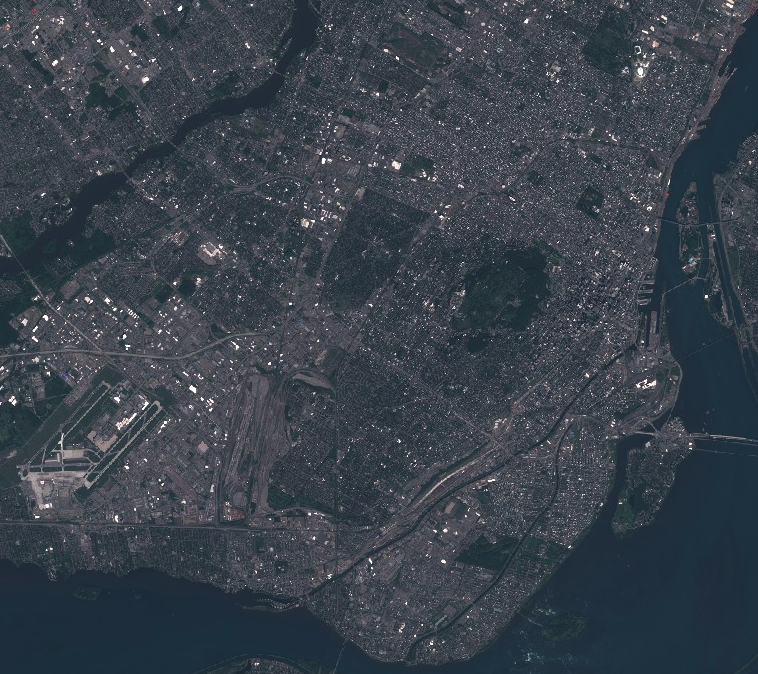
\includegraphics[width=.75\textwidth]{images/montreal_satellite}
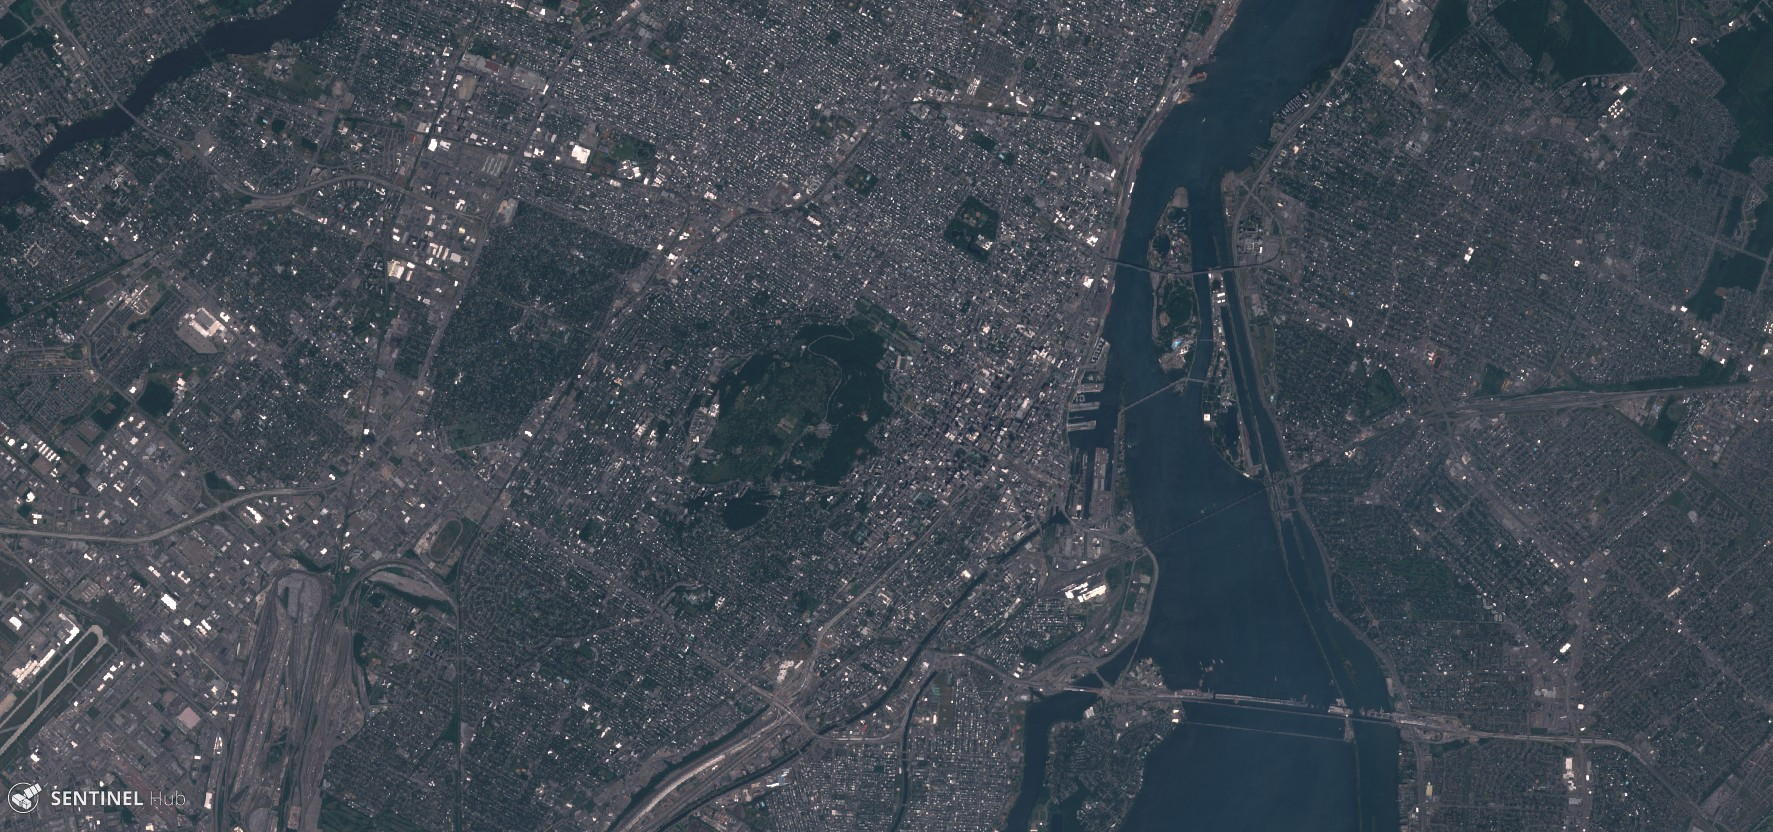
\includegraphics[width=\textwidth]{images/cloudfree}
\end{frame}

\begin{frame}
	\frametitle{Cloud coverage is very common}
		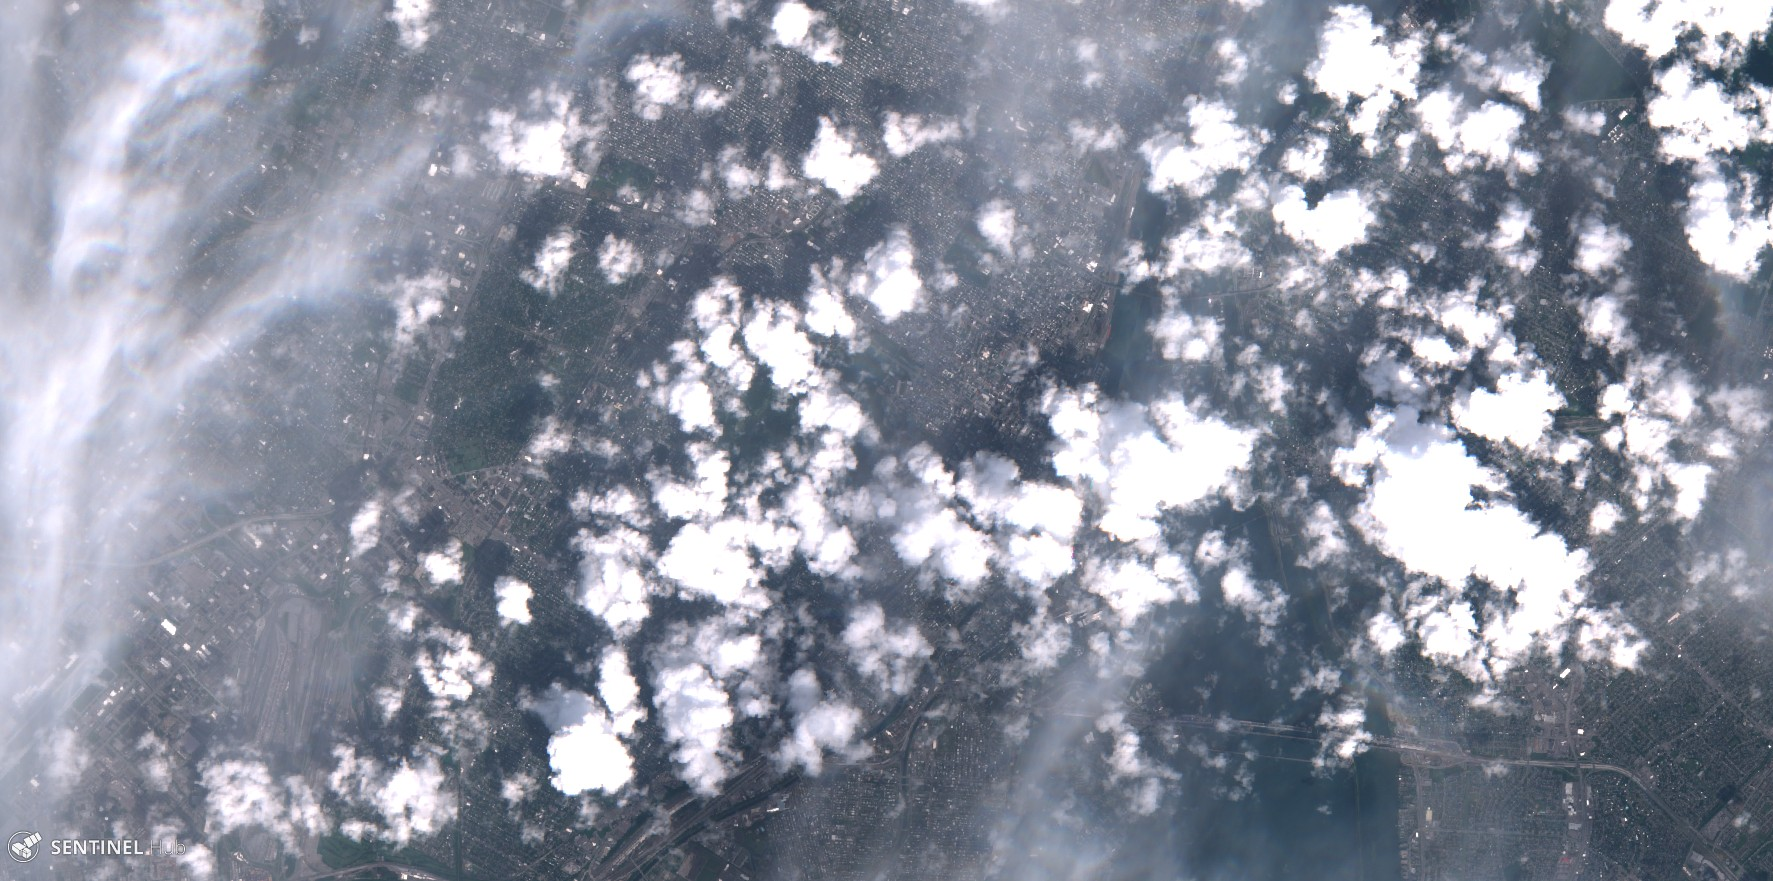
\includegraphics[width=\textwidth]{images/clouds}
	
%		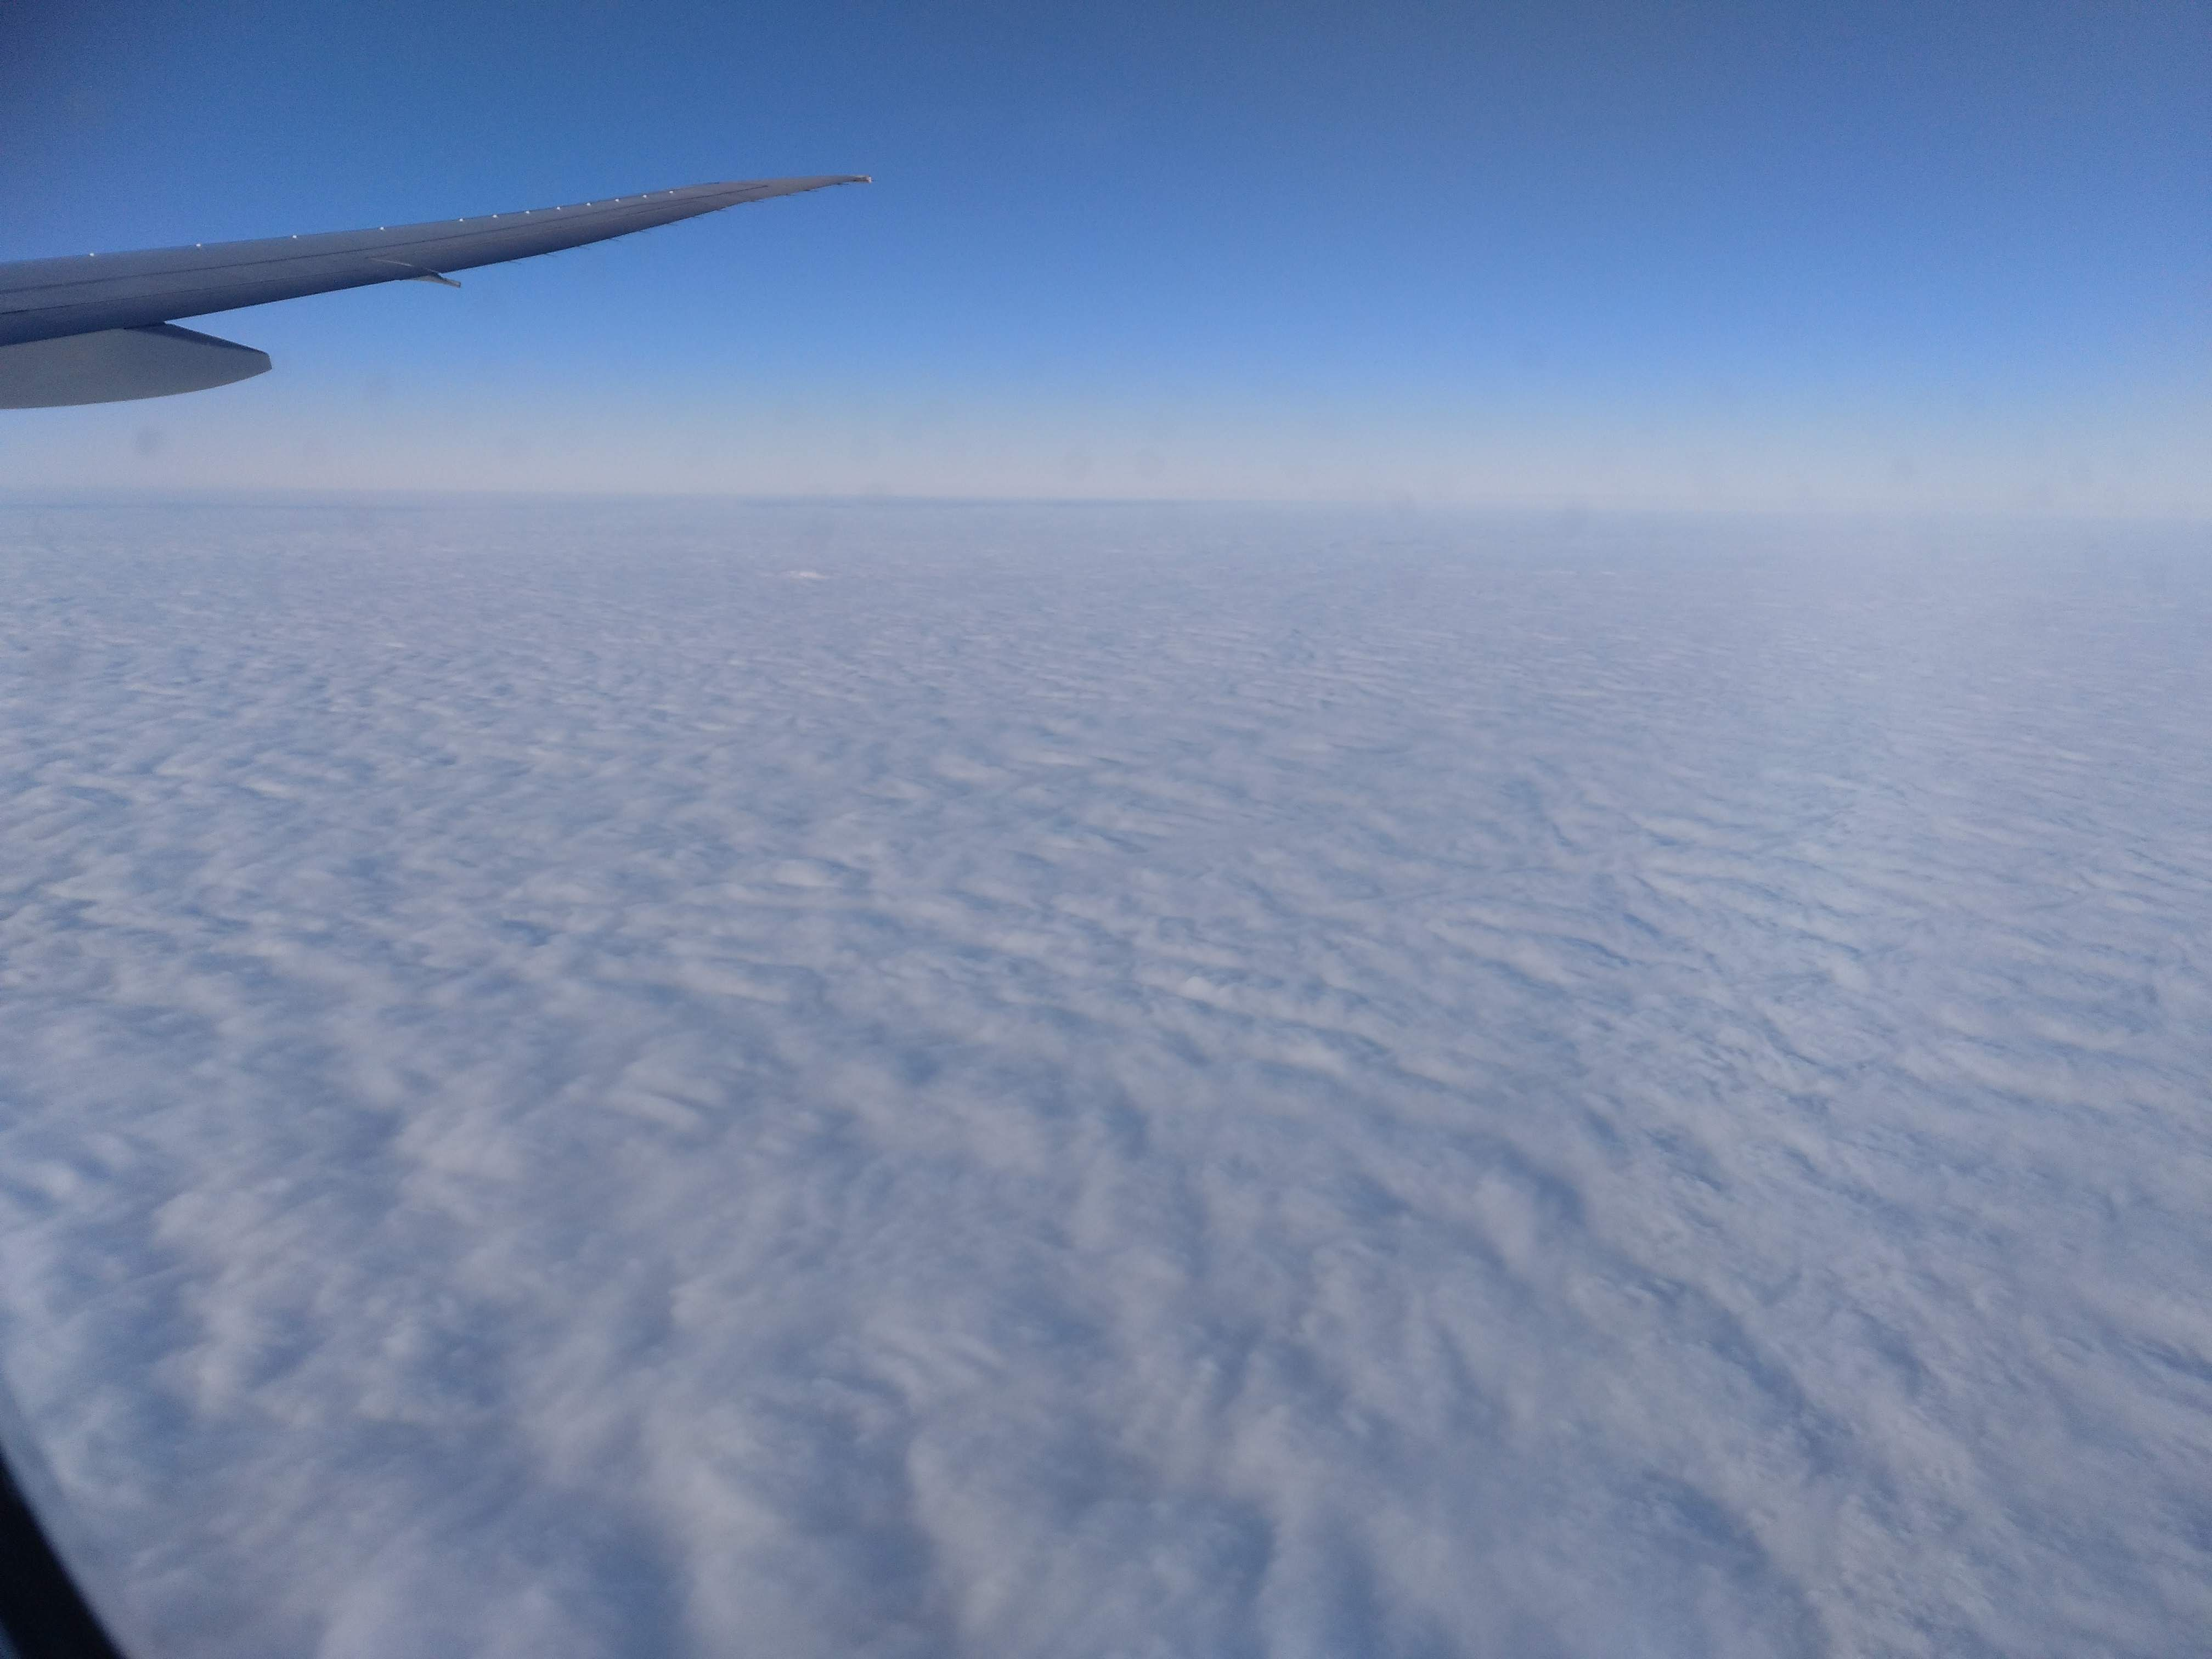
\includegraphics[width=\textwidth]{images/cloud_airplane}
		
\end{frame}

\begin{frame}
	\frametitle{Cloud coverage as spatiotemporal noise}
	\centering
	
	\def\imagewidth{1.5cm}
	
	
\includegraphics[width=\imagewidth]{images/activations/16494/x/x-0.png}
	
\includegraphics[width=\imagewidth]{images/activations/16494/x/x-1.png}
	
\includegraphics[width=\imagewidth]{images/activations/16494/x/x-2.png}
	
\includegraphics[width=\imagewidth]{images/activations/16494/x/x-3.png}
	
\includegraphics[width=\imagewidth]{images/activations/16494/x/x-4.png}
	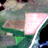
\includegraphics[width=\imagewidth]{images/activations/16494/x/x-5.png}
	
\includegraphics[width=\imagewidth]{images/activations/16494/x/x-6.png}
	
\includegraphics[width=\imagewidth]{images/activations/16494/x/x-7.png}
	
\includegraphics[width=\imagewidth]{images/activations/16494/x/x-8.png}
	
\includegraphics[width=\imagewidth]{images/activations/16494/x/x-9.png}
	
\includegraphics[width=\imagewidth]{images/activations/16494/x/x-10.png}
	
\includegraphics[width=\imagewidth]{images/activations/16494/x/x-11.png}
	
\includegraphics[width=\imagewidth]{images/activations/16494/x/x-12.png}
	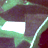
\includegraphics[width=\imagewidth]{images/activations/16494/x/x-13.png}
	
\includegraphics[width=\imagewidth]{images/activations/16494/x/x-14.png}
	
\includegraphics[width=\imagewidth]{images/activations/16494/x/x-15.png}
	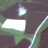
\includegraphics[width=\imagewidth]{images/activations/16494/x/x-16.png}
	
\includegraphics[width=\imagewidth]{images/activations/16494/x/x-18.png}
	
\includegraphics[width=\imagewidth]{images/activations/16494/x/x-19.png}
	
\includegraphics[width=\imagewidth]{images/activations/16494/x/x-20.png}
	
\includegraphics[width=\imagewidth]{images/activations/16494/x/x-21.png}
	
\includegraphics[width=\imagewidth]{images/activations/16494/x/x-22.png}
	
\includegraphics[width=\imagewidth]{images/activations/16494/x/x-23.png}
	
\includegraphics[width=\imagewidth]{images/activations/16494/x/x-24.png}
	
\includegraphics[width=\imagewidth]{images/activations/16494/x/x-25.png}
	
\includegraphics[width=\imagewidth]{images/activations/16494/x/x-26.png}
	
\includegraphics[width=\imagewidth]{images/activations/16494/x/x-27.png}
	
\includegraphics[width=\imagewidth]{images/activations/16494/x/x-28.png}
	
\includegraphics[width=\imagewidth]{images/activations/16494/x/x-29.png}
	
\includegraphics[width=\imagewidth]{images/activations/16494/x/x-30.png}
	
\includegraphics[width=\imagewidth]{images/activations/16494/x/x-31.png}
	
\includegraphics[width=\imagewidth]{images/activations/16494/x/x-32.png}
	
\includegraphics[width=\imagewidth]{images/activations/16494/x/x-33.png}
%	
\includegraphics[width=\imagewidth]{images/activations/16494/x/x-34.png}
%	
\includegraphics[width=\imagewidth]{images/activations/16494/x/x-35.png}
%	
\end{frame}
%
%\begin{frame}
%\LARGE
%\centering
%\textbf{Filter this temporal noise by pre-classificaition?}
%\end{frame}

%\begin{frame}
%		
\usepgfplotslibrary{groupplots}

\tikzsetnextfilename{scl}
\begin{tikzpicture}

%\def\data{images/classhist/classHistograms.dat}
\def\data{images/clouds/scl2.csv}

\pgfplotsset{ every non boxed x axis/.append style={x axis line style=-},
	every non boxed y axis/.append style={y axis line style=-}}

\pgfplotsset{every axis/.append style={ybar=1pt, bar width=6pt, ymajorgrids}}
\pgfplotsset{every axis label/.append style={font=\footnotesize},tick pos=left,ylabel near ticks}
\pgfplotsset{every tick label/.append style={font=\scriptsize}}
\pgfplotsset{every x tick label/.append style={rotate=90,anchor=east,font=\tiny}}
%   \pgfplotsset{every y tick label/.append style={/pgf/number format/.cd, fixed, precision=2, fixed zerofill,}}
%\tikzstyle{caption}=[font=\footnotesize, fill=tumwhite, fill opacity=.5, text opacity=1]


\begin{axis}[
%group style={
%	%       group size=1 by 4,
%	group size=1 by 1,
%	xlabels at=edge bottom,
%	xticklabels at=edge bottom,
%	ylabels at=edge left,
%	yticklabels at=edge left,
%	vertical sep=2pt,
%	horizontal sep=2pt
%},
width=\textwidth,
height=5cm,
%ymode=log,
%log origin=infty,
%     y dir=reverse,
%     scaled ticks=true,
%log ticks with fixed point,
%scaled x ticks=true,
axis lines=left,
xlabel={image acquisition dates},
ylabel={cloud coverage},
xlabel style={yshift=-2mm},
xmin=-.5,
xmax=46,
%xlabel=clouds,
ytick={1,10,25,50,100},
yticklabels={\SI{1}{\percent},\SI{10}{\percent},\SI{25}{\percent},\SI{50}{\percent},\SI{100}{\percent}},
xtick=data,
xticklabels={
	03. Jan,
	13. Jan,
	20. Jan,
	21. Jan,
	28. Jan,
	12. Feb,
	11. Mär,
	20. Mär,
	23. Mär,
	03. Apr,
	13 Apr.,
	19. Apr,
	22. Apr,
	29. Apr,
	02. Mai,
	10. Mai,
	22. Mai,
	29. Mai,
	08. Jun,
	18. Jun,
	28. Jan,
	02. Jul,
	14. Jul,
	18. Jul,
	21. Jul,
	28. Jul,
	30. Jul,
	07. Aug,
	17. Aug,
	20. Aug,
	28. Aug,
	21. Aug,
	09. Sep.,
	12. Sep..,
	18. Sep.,
	26. Sep.,
	29. Sep.,
	09. Okt.,
	18. Okt.,
	28. Okt.,
	09. Nov.,
	15. Nov.,
	18. Nov.,
	28. Nov.,
	06. Dez.,
	08. Dez.
},
axis on top
];

\addplot[
%       draw=tumblue,
draw=none,
fill=tumblue,rounded corners=.5pt
] table [col sep=comma, x=id, y=cloudpercent] {\data};


\end{axis}
\end{tikzpicture}
%\end{frame}



\tikzstyle{conn}=[-stealth, thick]
\tikzstyle{process}=[draw=none, rounded corners,text depth=0pt]

\newcommand{\figourapproach}{
\begin{tikzpicture}[node distance=2em]
\node[process](inputs){cloudy images $\V{x}$};
\node[process,right=5em of inputs](approach){prediction $\V{y}$};
\draw[conn] (inputs) -- node[midway, above]{$f(\V{x})$}(approach);

%\node[noteannot, above left= 1em and 2em of approach](annottext){\textbf{We treat clouds as data-inherent noise:}\\ by employing ConvLSTMs to learn cloud masking \\ and classification in \textbf{one model end-to-end}.};
%\draw[annotation] (annottext) -- (approach);
\end{tikzpicture}
}

\newcommand{\figcloudfilteringpipeline}{
\begin{tikzpicture}[node distance=2em]
\node[process](inputs){cloudy images $\V{x}$};
\visible<2>{\node[process,right=5em of inputs](approach){prediction $\V{y}$};}
\node[process](cloudclass) at ($ (inputs)!0.5!(approach) + (0,4em) $) {cloud mask $\V{m}$};

%\node[noteannot, above right= 1em and -3.5em of approach](annottext){\textbf{The pre-classification of clouds}\\requires \textbf{two separate models} \\ for cloud classification $f_{cl}$ and prediction $f$.};
%
%\draw[annotation] (annottext) -- (approach);
%\draw[annotation] (annottext) -- (cloudclass);

\draw[conn] (inputs) -- node[midway, above left]{$f_{cl}(\V{x})$}(cloudclass);

\visible<2>{
	\draw[conn] (inputs) -- node[at end, above]{$f(\V{x},\V{m})$}(approach);
	\draw[conn, rounded corners=11pt] (cloudclass) |- node[near end, above]{}(approach);
}
\end{tikzpicture}
}

\begin{frame}<presentation:0>

\frametitle{Detecting Clouds is rarely the main objective}
\LARGE
\centering\figcloudfilteringpipeline

\end{frame}

%


%\begin{frame}<presentation:1>
%
%\frametitle{Introducing a model to pre-classify clouds?}
%\LARGE
%\centering\figcloudfilteringpipeline
%
%\end{frame}

%\begin{frame}
%\frametitle{Clouds classification works very well...}
%
%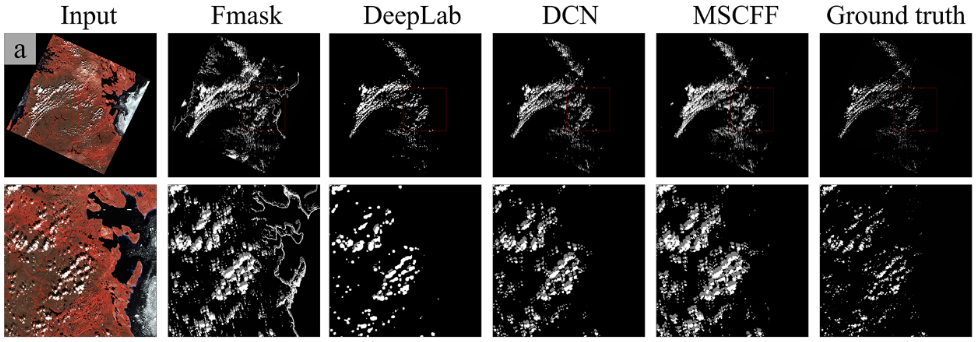
\includegraphics[width=\textwidth]{images/Li18_clouds}
%
%\texttt{\small Li, Z., Shen, H., Cheng, Q., Liu, Y., You, S., \& He, Z. (2018). Deep learning based cloud detection for remote sensing images by the fusion of multi-scale convolutional features. arXiv preprint arXiv:1810.05801.}
%\end{frame}
%
%\begin{frame}<presentation:2>
%
%\frametitle{Identifying clouds is rarely the main objective!}
%\LARGE
%\centering\figcloudfilteringpipeline
%
%\end{frame}


\begin{frame}
\frametitle{End-to-end trainable model for robust classification}
\LARGE
\centering\figourapproach		

\end{frame}


\def\fps{3}
%\tikzsetnextfilename{lstm}

\tikzstyle{operator} = [draw, circle, fill=tumbluemedium, draw=tumbluemedium, inner sep=0, text=white]
%\tikzstyle{function} = [draw, rectangle, fill=tumbluemedium, draw=tumbluemedium, text=white]
\tikzstyle{gate} = [fill=tumivory,draw,rounded corners=1pt, inner sep=2pt, minimum width=11mm, minimum height=11mm]
\tikzstyle{io} = [fill=tumwhite,draw,rounded corners=1pt, inner sep=2pt, minimum width=11mm, minimum height=11mm]

\tikzstyle{dummy} = [inner sep=0]
\tikzstyle{flow} = [rounded corners]
\tikzstyle{endflow} = [-stealth,flow]

\colorlet{boxcolor}{tumgraylight}
\tikzstyle{bigbox} = [rectangle, draw=tumivory, thick, fill=boxcolor, rounded corners, 
inner xsep=0ex, inner ysep=2ex]

\tikzset{pic shift/.store in=\shiftcoord,
	pic shift={(0,0)},
	lstmexplain/.pic = {
		\begin{scope}[shift={\shiftcoord},xscale=6,yscale=2.5]
			
			\node[dummy] (bl) at (0,0){}; % bottom left
			\node[dummy] (tr) at (1,1){}; % top right
			
			\node[dummy] (br) at ($ (bl -| tr) $){}; % bottom right
			\node[dummy] (tl) at ($ (bl |- tr) $){}; % top left
			
			\node[fit=(bl) (tr),bigbox] (-C) {};
			
			% input coordinate for rounded draw lines -> slightly right of tl
			\coordinate (-input) at (0.1,1); % top left
			
			% output coordinate for rounded draw lines -> slightly left of br
			\coordinate (-coutput) at (0.98,0); % bottom right
			\coordinate (-houtput) at (0.98,1); % bottom right
			
%			% gate distance
			\def\d{1/5}
			
			% gate heights
			\def\h{1/3}
			
			\coordinate (f)  at bl+(0.7*\d,0);
			\coordinate (i)  at bl+(1.8*\d,0);
			\coordinate (j)  at bl+(2.9*\d,0);
			\coordinate (o)  at bl+(4*\d,0);
			\coordinate (out) at bl+(4.7*\d,0);
			
			\coordinate (gates) at (0,2*\h);
			
			%\node[above=of tl](xt){$x_{t}$};
			%\node[left=of tl](htminus1){$h_{t-1}$};
			
			%\node[below=of br](ct){$c_{t}$};
%			\setlength{\thinmuskip}{0pt}
			
			\visible<2->{
			\node[gate](fgate) at ($ (gates -| f) $){
				$\VForgetGate_t$
				};
				\draw[endflow] (-input) -| (fgate);
			}
			
			\visible<3->{
			\node[gate](igate) at ($ (gates -| i) $){
				$\VInputGate_t$
				};
			}
				
			\visible<3->{
			\node[gate](jgate) at ($ (gates -| j) $){$\VModulationGate_t$};
			\node[operator](jmult) at ([shift={(0,-1.3*\h)}]jgate) {$ \odot $};
			\draw[endflow] (-input) -| (jgate);
			\draw[endflow] (jgate) -- (jmult);
			\draw[endflow] (-input) -| (igate); 
			\draw[endflow] (igate) |- (jmult);
			}
				
			\visible<4->{
			\node[gate](ogate) at ($ (gates -| o) $){
				$\VOutputGate_t$
				};
			\draw[endflow] (tl) -| (ogate);
			}
			
%			\coordinate (htminus1) at bl+(-.5,0);
%			\coordinate (ht) at bl+(-.5,0);
%			
			% forget gate 
			\visible<5->{
			\node[operator](fmult) at ($ (bl -| fgate) $) {$ \odot $};
			\draw[endflow] (fgate) -- (fmult); 
			\node[operator](cadd) at ($ (bl -| jgate) $) {$ + $};
			\draw[endflow] (jmult) -- (cadd); 
			\draw[flow] (fmult) -- (cadd) -- (-coutput);		
			}

			\visible<6->{
			\node[operator](outtanh) at ($ (jmult -| out) $) {$\odot$};
			\draw[endflow] (ogate) |- (outtanh);
			\draw[flow] (outtanh) |- (-houtput);
			\draw[endflow] (cadd) -| (outtanh);
			}
		\end{scope}
	}
}

\tikzset{pic shift/.store in=\shiftcoord,
	pic shift={(0,0)},
	lstmanim/.pic = {
		\begin{scope}[shift={\shiftcoord},xscale=6,yscale=2.5]
			
			\node[dummy] (bl) at (0,0){}; % bottom left
			\node[dummy] (tr) at (1,1){}; % top right
			
			\node[dummy] (br) at ($ (bl -| tr) $){}; % bottom right
			\node[dummy] (tl) at ($ (bl |- tr) $){}; % top left
			
			\node[fit=(bl) (tr),bigbox] (-C) {};
			
			% input coordinate for rounded draw lines -> slightly right of tl
			\coordinate (-input) at (0.1,1); % top left
			
			% output coordinate for rounded draw lines -> slightly left of br
			\coordinate (-coutput) at (0.98,0); % bottom right
			\coordinate (-houtput) at (0.98,1); % bottom right
			
			%			% gate distance
			\def\d{1/5}
			
			% gate heights
			\def\h{1/3}
			
			\coordinate (f)  at bl+(0.7*\d,0);
			\coordinate (i)  at bl+(1.8*\d,0);
			\coordinate (j)  at bl+(2.9*\d,0);
			\coordinate (o)  at bl+(4*\d,0);
			\coordinate (out) at bl+(4.7*\d,0);
			
			\coordinate (gates) at (0,2*\h);
			
			%\node[above=of tl](xt){$x_{t}$};
			%\node[left=of tl](htminus1){$h_{t-1}$};
			
			%\node[below=of br](ct){$c_{t}$};
			
			\node[gate, label={[label distance=0ex]265:$\VForgetGate_{t}$}](fgate) at ($ (gates -| f) $){
				\animategraphics[poster=25,width=1cm,autoplay,loop]{\fps}{images/activations/16494/f/3-}{1}{36}
				};
			\node[gate, label={[label distance=0ex]265:$\VInputGate_{t}$}](igate) at ($ (gates -| i) $){
				\animategraphics[poster=25,width=1cm,autoplay,loop]{\fps}{images/activations/16494/i/3-}{1}{36}
				};
			\node[gate, label={[label distance=0ex]265:$\VModulationGate_{t}$}](jgate) at ($ (gates -| j) $){
				\animategraphics[poster=25,width=1cm,autoplay,loop]{\fps}{images/activations/16494/j/3-}{1}{36}
				};
			\node[gate, label={[label distance=0ex]265:$\VOutputGate_{t}$}](ogate) at ($ (gates -| o) $){
				\animategraphics[poster=25,width=1cm,autoplay,loop]{\fps}{images/activations/16494/o/3-}{1}{36}
				};
			
			%			\coordinate (htminus1) at bl+(-.5,0);
			%			\coordinate (ht) at bl+(-.5,0);
			%			
			% forget gate
			\node[operator](fmult) at ($ (bl -| fgate) $) {$ \odot $};
			\draw[endflow] (-input) -| (fgate);
			\draw[endflow] (fgate) -- (fmult); 
			
			%			%j
			\node[operator](jmult) at ([shift={(0,-1.3*\h)}]jgate) {$ \odot $};
			\node[operator](cadd) at ($ (bl -| jgate) $) {$ + $};
			\draw[endflow] (-input) -| (jgate);
			\draw[endflow] (jgate) -- (jmult);
			\draw[endflow] (jmult) -- (cadd); 			
			
			%			%i	
			\draw[endflow] (-input) -| (igate);
			\draw[endflow] (igate) |- (jmult); 
			%
			%%			% outpu
			\node[operator](outtanh) at ($ (jmult -| out) $) {$\odot$};
			%			
			%			%o 
			\draw[endflow] (tl) -| (ogate);
			\draw[endflow] (ogate) |- (outtanh);
			\draw[flow] (outtanh) |- (-houtput);
			%			
			%			% output flow
			\draw[endflow] (cadd) -| (outtanh);
			\draw[flow] (fmult) -- (cadd) -- (-coutput);
			%			
			
		\end{scope}
	}
}

\tikzset{pic shift/.store in=\shiftcoord,
	pic shift={(0,0)},
	simplernn/.pic = {
		\begin{scope}[shift={\shiftcoord},xscale=2,yscale=.1]
			
			\node[dummy] (bl) at (0,0){}; % bottom left
			\node[dummy] (tr) at (1,1){}; % top right
			
			\node[dummy] (br) at ($ (bl -| tr) $){}; % bottom right
			\node[dummy] (tl) at ($ (bl |- tr) $){}; % top left
			
			\node[fit=(bl) (tr),bigbox] (-C) {};
			
			% input coordinate for rounded draw lines -> slightly right of tl
			\coordinate (-input) at (0.1,1); % top left
			
			% output coordinate for rounded draw lines -> slightly left of br
			\coordinate (-coutput) at (0.98,0); % bottom right
			\coordinate (-houtput) at (0.98,1); % bottom right
			
			%			% gate distance
			\def\d{1/5}
			
			% gate heights
			
			\node[] at ($ (-input)!0.5!(-houtput) $)(label){
				RNN
%				$\sigma(\concat{\VInput_t}{\VHidden_{t-1}}\MWeight$
			};
			\draw[endflow] (-input) -- (label);
			\draw[flow] (label) -- (-houtput);
			%\node[above=of tl](xt){$x_{t}$};
			%\node[left=of tl](htminus1){$h_{t-1}$};
			
			%\node[below=of br](ct){$c_{t}$};
			
%			\node[gate, label={[label distance=0ex]265:$\VForgetGate_{t}$}](fgate) at ($ (gates -| f) $){
%				\animategraphics[poster=25,width=1cm,autoplay,loop]{\fps}{images/activations/16494/f/3-}{1}{36}
%			};
%			\node[gate, label={[label distance=0ex]265:$\VInputGate_{t}$}](igate) at ($ (gates -| i) $){
%				\animategraphics[poster=25,width=1cm,autoplay,loop]{\fps}{images/activations/16494/i/3-}{1}{36}
%			};
%			\node[gate, label={[label distance=0ex]265:$\VModulationGate_{t}$}](jgate) at ($ (gates -| j) $){
%				\animategraphics[poster=25,width=1cm,autoplay,loop]{\fps}{images/activations/16494/j/3-}{1}{36}
%			};
%			\node[gate, label={[label distance=0ex]265:$\VOutputGate_{t}$}](ogate) at ($ (gates -| o) $){
%				\animategraphics[poster=25,width=1cm,autoplay,loop]{\fps}{images/activations/16494/o/3-}{1}{36}
%			};
			
			%			\coordinate (htminus1) at bl+(-.5,0);
			%			\coordinate (ht) at bl+(-.5,0);
			%			
			% forget gate
%			\node[operator](fmult) at ($ (bl -| fgate) $) {$ \odot $};
%			\draw[endflow] (-input) -| (fgate);
%			\draw[endflow] (fgate) -- (fmult); 
			
			%			%j
%			\node[operator](jmult) at ([shift={(0,-1.3*\h)}]jgate) {$ \odot $};
%			\node[operator](cadd) at ($ (bl -| jgate) $) {$ + $};
%			\draw[endflow] (-input) -| (jgate);
%			\draw[endflow] (jgate) -- (jmult);
%			\draw[endflow] (jmult) -- (cadd); 			
			
			%			%i	
%			\draw[endflow] (-input) -| (igate);
%			\draw[endflow] (igate) |- (jmult); 
			%
			%%			% outpu
%			\node[operator](outtanh) at ($ (jmult -| out) $) {$\odot$};
			%			
			%			%o 
%			\draw[endflow] (tl) -| (ogate);
%			\draw[endflow] (ogate) |- (outtanh);
%			\draw[flow] (outtanh) |- (-houtput);
			%			
			%			% output flow
%			\draw[endflow] (cadd) -| (outtanh);
%			\draw[flow] (fmult) -- (cadd) -- (-coutput);
			%			
			
		\end{scope}
	}
}

\tikzset{pic shift/.store in=\shiftcoord,
	pic shift={(0,0)},
	gru/.pic = {
		\begin{scope}[shift={\shiftcoord},xscale=6,yscale=2.5]
			
			\node[dummy] (bl) at (0,0){}; % bottom left
			\node[dummy] (tr) at (1,1){}; % top right
			
			\node[dummy] (br) at ($ (bl -| tr) $){}; % bottom right
			\node[dummy] (tl) at ($ (bl |- tr) $){}; % top left
			
			\node[fit=(bl) (tr),bigbox] (-C) {};
			
			%			% gate distance
			\def\d{1/5}
			
			% gate heights
			\def\h{1/4}
			
			
			% input coordinate for rounded draw lines -> slightly right of tl
			\coordinate (-xinput) at (0.3*\d,1); % top left
			\coordinate (-xinputflow) at (0.5*\d,1); % top left
			
			\coordinate (-hinput) at (0.2*\d,1); % top left
			\coordinate (-hinputflow) at (0.2*\d,.9); % top left
			
			% output coordinate for rounded draw lines -> slightly left of br
			\coordinate (-houtput) at (.98,1); % bottom right
			
			\coordinate (r)  at bl+(1*\d,0);
			\coordinate (rgap)at bl+(2*\d,0);
			\coordinate (u)  at bl+(3*\d,0);
			\coordinate (c)  at bl+(4*\d,0);
			
			\coordinate (out) at bl+(4.75*\d,0);
			
			\coordinate (abovegates) at (0,3.5*\h);
			\coordinate (gates) at (0,2.3*\h);
			\coordinate (belowgates) at ($(gates)!0.65!(bl)$);
			
			
%			\node[above=of tl](xt){$x_{t}$};
%			\node[left=of tl](htminus1){$h_{t-1}$};
			
			%\node[below=of br](ct){$c_{t}$};
			
			
			\node[gate](rgate) at ($ (gates -| r) $){r};
			\node[gate](ugate) at ($ (gates -| u) $){u};
			\node[gate](cgate) at ($ (gates -| c) $){$\tilde{\VHidden}$};
			
			\node[operator](cadd) at ($ (cgate |- bl) $) {$+$};
			\node[operator](cmult) at ($ (cgate |- belowgates) $) {$\odot$};
			
			\node[operator](rmult) at ($ (rgap |- belowgates) $) {$\odot$};
			
			\node[operator](umult) at ($ (u |- bl) $) {$\odot$};
			\draw[endflow] (ugate) -- (umult); 
			
			\draw[endflow] (-hinput)++(0,-.1) |- ($ (bl -| rgate) $) -| (rmult); 
			\draw[endflow] (rgate) |- (rmult);
			
			\draw[endflow] (cgate) -- (cmult);
			\draw[endflow] (ugate) |- (cmult);
			\draw[endflow] (cmult) -- (cadd);
			
			
			%%			
			\draw[endflow] (-xinputflow) -| (rgate); 
			\draw[endflow] (-xinputflow) -| ($ (rgate |- abovegates) $) -| (ugate); 
%%			\draw[endflow] (rgate) |- ++(.5\d,-\h) -| (rgate); 
			
			\draw[flow, draw=boxcolor,double=black,double distance=\pgflinewidth,ultra thick] (rmult) |- ($ (ugate |- tl) $);
			
			
			%\draw[flow] (tl) |- ($ (abovegates -| u) $) -| (ugate); 
			\draw[endflow] (-xinputflow) -| (cgate); 
			\draw[flow] (-hinput)++(-0.1, 0) -- (-xinputflow); 
			
			\draw[flow] (-hinputflow) |- (umult) -- (cadd) -| ($ (out) + (0,.5) $) |- (-houtput); %($(br)!0.5!(tr)$) 
			
			
			
			%% debug
%			\node at (gates) {\tiny{gates}};
%			\node at (abovegates) {\tiny{abovegates}};
%			\node at (belowgates) {\tiny{belowgates}};
%			\node at (-input) {\tiny{-input}};
%			\node at (-coutput) {\tiny{-coutput}};
%			\node at (-houtput) {\tiny{-houtput}};
%			\node at (f) {\tiny{f}};
%			\node at (i) {\tiny{i}};
%			\node at (j) {\tiny{j}};
%			\node at (o) {\tiny{o}};
%			\node at (tl) {\tiny{tl}};
%			\node at (br) {\tiny{br}};
%			\node at (bl) {\tiny{bl}};
%			\node at (tr) {\tiny{tr}};
%			\node at (out) {\tiny{out}};
			
		\end{scope}
	}
}

\tikzset{pic shift/.store in=\shiftcoord,
	pic shift={(0,0)},
	concat/.pic = {
		\node[](a) at (0, .5){$\V{a}$};
		\node[](b) at (0, -.5){$\V{b}$};
		\node[](out) at (1, 0){$\concat{ \V{a} }{ \V{b} }$};
		
		\draw[endflow] (a) |- (out);
		\draw[endflow] (b) |- (out);
	}
}

\tikzset{pic shift/.store in=\shiftcoord,
	pic shift={(0,0)},
	copy/.pic = {
		\node[](ain) at (0, 0){$\V{a}$};
		\node[](aout1) at (.5, .5){$\V{a}$};
		\node[](aout2) at (.5, -.5){$\V{a}$};
		\draw[endflow] (ain) -| (aout1);
		\draw[endflow] (ain) -| (aout2);
	}
}

\tikzset{pic shift/.store in=\shiftcoord,
	pic shift={(0,0)},
	fgate/.pic = {
		\begin{scope}[shift={\shiftcoord},xscale=1,yscale=1]
			
			\node[dummy] (tl_a) at (0,0){}; % bottom left
			\node[dummy] (br_a) at (1,1){}; % top right
			
			\node[fit=(br_a) (tr_a),gate,inner sep=0] (-C) {};
			
			\node[draw] (conv) at (0.5,0){$conv$}; % bottom left
			\node[draw] (bn) at (0.5,.5){$bn$}; % bottom left
			\node[draw] (sigmoid) at (0.5,1){$\sigma$}; % bottom left
				
		\end{scope}
	}
}

\newcommand{\gru}{
\begin{tikzpicture}[scale=1, node distance=2em]%,show background rectangle,background rectangle/.style={draw=red}]
\draw pic (GRU) at (0,0) {gru};
\node[io,left=of GRU-hinput](gru_htminus1){$\VHidden_{t-1}$};
\draw[rounded corners] (gru_htminus1) -| (GRU-hinputflow);
\node[io,above=of GRU-xinput](gru_xt){$\VInput_{t}$};

\draw[rounded corners] (gru_xt) |- (GRU-xinputflow);

\node[io,right=of GRU-houtput](gru_ht){$\VHidden_{t}$};
\draw[rounded corners] (GRU-houtput)--(gru_ht);
\end{tikzpicture}
}

\newcommand{\lstmexplain}{
	\begin{tikzpicture}[scale=1, node distance=2em]%,show background rectangle,background rectangle/.style={draw=red}]
	
	
	%\clip(0,0) rectangle (7,7);
	
	%\draw pic (B) at (5,0) {lstm};
	
	%\draw pic (C) at (10,0) {lstm};
	
	%\draw pic (C) at (2,2) {fgate};
	
	\draw pic (LSTM) at (0,0) {lstmexplain};
	\node[io,xshift=1ex,above=3em of LSTMtl, label=above:\phantom{$\VInput_{t}$}](xt){$\VInput_{t}$};%$x_{t}$
		
	\node[io,left=of LSTMtl](htminus1){$\VHidden_{t-1}$};
	
	\node[io,right=of LSTMbr](ct){$\VCellState_{t}$}; % $c_{t}$

	\node[io,left=of LSTMbl](ctminus1){$\VCellState_{t-1}$}; % 
		
	\node[io,right=of LSTMtr](ht){$\VHidden_{t}$};
	
	%% iterative connections
	\visible<7->{
	\draw[endflow] (ct) -- ($ (ct)+(0,-0.8) $) -| (ctminus1);
	\draw[endflow] (ht) -- ($ (ht)+(0,.8) $) -| (htminus1);
	}
		
	\visible<2->{
	\draw[rounded corners] (xt) |- (LSTM-input);
	}
	

	\visible<2->{
	\draw[endflow] (htminus1) -- (LSTM-input);
	}
	
	\visible<5->{
	\draw[endflow] (LSTM-coutput)--(ct);
	}
	
	
	\visible<5->{
	\draw[endflow] (ctminus1)--(LSTMfmult);
	}
	
	\visible<6->{
	\draw[endflow] (LSTM-houtput)--(ht);
	}
	\end{tikzpicture}
}

\newcommand{\lstmanim}{
	\begin{tikzpicture}[scale=1, node distance=2em]%,show background rectangle,background rectangle/.style={draw=red}]
	
	
	\draw pic (LSTM) at (0,0) {lstmanim};
	\node[io,xshift=1ex,above=3em of LSTMtl, ,label=above:$\VInput_{t}$](xt){\animategraphics[poster=25,width=1cm,autoplay,loop]{\fps}{images/activations/16494/x/x-}{1}{36}};%$x_{t}$
	\draw[rounded corners] (xt) |- (LSTM-input);
	\node[io,left=of LSTMtl,label=below:$\VHidden_{t-1}$](htminus1){
		\animategraphics[poster=24,width=1cm,autoplay,loop]{\fps}{images/activations/16494/output/3-}{0}{35}
	};
	\draw[endflow] (htminus1) -- (LSTM-input);
	\node[io,right=of LSTMbr,label=above:$\VCellState_{t}$](ct){\animategraphics[poster=25,width=1cm,autoplay,loop]{\fps}{images/activations/16494/state/3-}{1}{36}}; % $c_{t}$
	\draw[endflow] (LSTM-coutput)--(ct);
	\node[io,left=of LSTMbl,label=above:$\VCellState_{t-1}$](ctminus1){\animategraphics[poster=24,width=1cm,autoplay,loop]{\fps}{images/activations/16494/state/3-}{0}{35}}; % 
	\draw[endflow] (ctminus1)--(LSTMfmult);
	\node[io,right=of LSTMtr,label=below:$\VHidden_{t}$](ht){
		\animategraphics[poster=24,width=1cm,autoplay,loop]{\fps}{images/activations/16494/output/3-}{1}{36}
	};
	\draw[endflow] (LSTM-houtput)--(ht);
	
	\draw[endflow] (ct) -- ($ (ct)+(0,-0.8) $) -| (ctminus1);
	\draw[endflow] (ht) -- ($ (ht)+(0,.8) $) -| (htminus1);
	
	\end{tikzpicture}
}

\newcommand{\rnn}{
	\begin{tikzpicture}[scale=1, node distance=2em]%,show background rectangle,background rectangle/.style={draw=red}]
	
	
	\draw pic (RNN) at (0,0) {simplernn};
	\node[io,xshift=1ex,above=3em of RNNtl](xt){
		$\VInput_{t}$
%		\animategraphics[poster=25,width=1cm,autoplay,loop]{\fps}{images/activations/16494/x/x-}{1}{36}
	};%$x_{t}$
	\draw[rounded corners] (xt) |- (RNN-input);
	\node[io,left=of RNNtl](htminus1){
		$\VHidden_{t-1}$
%		\animategraphics[poster=24,width=1cm,autoplay,loop]{\fps}{images/activations/16494/output/3-}{0}{35}
	};
	\draw[flow] (htminus1) -- (RNN-input);
%	\node[io,right=of LSTMbr,label=above:$\VCellState_{t}$](ct){
%		\animategraphics[poster=25,width=1cm,autoplay,loop]{\fps}{images/activations/16494/state/3-}{1}{36}
%	}; % $c_{t}$
%	\draw[endflow] (LSTM-coutput)--(ct);
%	\node[io,left=of LSTMbl,label=above:$\VCellState_{t-1}$](ctminus1){
%		\animategraphics[poster=24,width=1cm,autoplay,loop]{\fps}{images/activations/16494/state/3-}{0}{35}
%	}; % 
%	\draw[endflow] (ctminus1)--(LSTMfmult);
	\node[io,right=of RNNtr](ht){
		$\VHidden_{t}$
%		\animategraphics[poster=24,width=1cm,autoplay,loop]{\fps}{images/activations/16494/output/3-}{1}{36}
	};
	\draw[endflow] (RNN-houtput)--(ht);
	
%	\draw[endflow] (ct) -- ($ (ct)+(0,-0.8) $) -| (ctminus1);
	\draw[endflow] (ht) -- ($ (ht)+(0,-.8) $) -| (htminus1);
	
	\end{tikzpicture}
}

\begin{frame}[t]
\frametitle{Extracting features from noisy data with ConvRNNs}

\centering
		%\lstmanim
		\begin{tikzpicture}[scale=1, node distance=2em]%,show background rectangle,background rectangle/.style={draw=red}]
		
		
		\draw pic (LSTM) at (0,0) {lstmanim};
		\node[io,xshift=1ex,above=3em of LSTMtl, ,label=above:$\VInput_{t}$](xt){\animategraphics[poster=25,width=1cm,autoplay,loop]{\fps}{images/activations/16494/x/x-}{1}{36}};%$x_{t}$
		\draw[rounded corners] (xt) |- (LSTM-input);
		\node[io,left=of LSTMtl,label=below:$\VHidden_{t-1}$](htminus1){
			\animategraphics[poster=24,width=1cm,autoplay,loop]{\fps}{images/activations/16494/output/3-}{0}{35}
		};
		\draw[endflow] (htminus1) -- (LSTM-input);
		\node[io,right=of LSTMbr,label=above:$\VCellState_{t}$](ct){\animategraphics[poster=25,width=1cm,autoplay,loop]{\fps}{images/activations/16494/state/3-}{1}{36}}; % $c_{t}$
		\draw[endflow] (LSTM-coutput)--(ct);
		\node[io,left=of LSTMbl,label=above:$\VCellState_{t-1}$](ctminus1){\animategraphics[poster=24,width=1cm,autoplay,loop]{\fps}{images/activations/16494/state/3-}{0}{35}}; % 
		\draw[endflow] (ctminus1)--(LSTMfmult);
		\node[io,right=of LSTMtr,label=below:$\VHidden_{t}$](ht){
			\animategraphics[poster=24,width=1cm,autoplay,loop]{\fps}{images/activations/16494/output/3-}{1}{36}
		};
		\draw[endflow] (LSTM-houtput)--(ht);
		
		\draw[endflow] (ct) -- ($ (ct)+(0,-0.8) $) -| (ctminus1);
		\draw[endflow] (ht) -- ($ (ht)+(0,.8) $) -| (htminus1);
		
		\end{tikzpicture}
	
\end{frame}

\begin{frame}<presentation:3>
	\frametitle{Employ ConvRNNs for Vegetation Land Cover Classification directly}
%	%\tikzsetnextfilename{network}

%\tikzstyle{operator} = [draw, circle, fill=tumbluemedium, draw=tumbluemedium, inner sep=0, text=white]
%\tikzstyle{function} = [draw, rectangle, fill=tumbluemedium, draw=tumbluemedium, text=white]
%\tikzstyle{gate} = [fill=tumivory,draw,rounded corners]

%\tikzstyle{dummy} = [inner sep=0]
\tikzstyle{flow} = [rounded corners, semithick]
\tikzstyle{endflow} = [-stealth,flow]
\tikzstyle{beginflow} = [stealth-,flow]
%\tikzstyle{perspective3drnn}=[z={(0.5cm,-0.5cm)}, x={(1cm,0cm)}, y={(0cm,1cm)}]
\tikzstyle{perspective3drnn}=[
x={(0.5cm,0.5cm)}, y={(1cm,0cm)}, z={(0cm,1cm)}]


\tikzstyle{bigpassbox} = [opacity=.2, rounded corners, draw=none]

\colorlet{focusone}{tumbluelight}
\colorlet{focustwo}{tumorange}

\colorlet{forwardcolor}{focusone}%tumbluemedium
\colorlet{backwardcolor}{focustwo}
\colorlet{classcolor}{tumivory}

% defaultvalue -> might be replaced later
\colorlet{tensorcolor}{forwardcolor}

\tikzstyle{bigbox} = [rectangle, draw=tumivory, thick, fill=tumblack!20, rounded corners, 
inner sep=.5ex]

\tikzstyle{wireframe} = [draw=tumgray]

\tikzstyle{image} = [inner sep=0, fill=none, minimum size=\imagewidth]

\tikzset{pic shift/.store in=\shiftcoord,
	pic shift={(0,0)},
	pics/seqlstmfw/.style={
		code={
		\begin{scope}[shift={\shiftcoord},xscale=3,yscale=2]
			
			\node[dummy] (bl) at (0,0){}; % bottom left
			\node[dummy] (tr) at (1,1){}; % top right
			
			\node[dummy] (br) at ($ (bl -| tr) $){}; % bottom right
			\node[dummy] (tl) at ($ (bl |- tr) $){}; % top left
			
			\node[fit=(bl) (tr),bigbox] (-C) {};
			
			% input coordinate for rounded draw lines -> slightly right of tl
			\coordinate (-input) at (0.1,1); % top left
			
			% output coordinate for rounded draw lines -> slightly left of br
			\coordinate (-coutput) at (0.9,0); % bottom right
			\coordinate (-cinput) at (0.1,0); % bottom left
			\coordinate (-houtput) at (0.9,1); % bottom right
			
%			% gate distance
			\def\d{1/6}
			
			% gate heights
			\def\h{1/3}
			
			\coordinate (f)  at bl+(1*\d,0);
			\coordinate (i)  at bl+(2*\d,0);
			\coordinate (j)  at bl+(3*\d,0);
			\coordinate (o)  at bl+(4*\d,0);
			\coordinate (out) at bl+(5*\d,0);
			
			\coordinate (gates) at (0,2*\h);
			
			%\node[above=of tl](xt){$x_{t}$};
			%\node[left=of tl](htminus1){$h_{t-1}$};
			
			%\node[below=of br](ct){$c_{t}$};
			
			\node[inner sep=0](fgate) at ($ (gates -| f) $){};
			\node[inner sep=0](igate) at ($ (gates -| i) $){};
			\node[inner sep=0](jgate) at ($ (gates -| j) $){};
			\node[inner sep=0](ogate) at ($ (gates -| o) $){};
			
%			\coordinate (htminus1) at bl+(-.5,0);
%			\coordinate (ht) at bl+(-.5,0);
%			
			% forget gate
			\node[operator](fmult) at ($ (bl -| fgate) $) {};
			\draw[endflow] (-input) -| (fgate) -- (fmult); 
			
%			%j
			\node[operator](jmult) at ([shift={(0,-1*\h)}]jgate) {};
			\node[operator](cadd) at ($ (bl -| jgate) $) {};
			\draw[endflow] (-input) -| (jgate) -- (jmult);
			\draw[endflow] (jmult) -- (cadd); 			

%			%i	
			\draw[endflow] (-input) -| (igate) |- (jmult); 
%
%%			% outpu
			\node[operator](outtanh) at ([shift={(0,1*\h)}]out) {};
%			
%			%o 
			\draw[endflow] (tl) -| (ogate) |- (outtanh);
			\draw[flow] (outtanh) |- (-houtput);
%			
%			% output flow
			\draw[endflow] (cadd) -| (outtanh);
			\draw[flow] (-cinput) -- (fmult) -- (cadd) -- (-coutput);
%			
		\end{scope}
		}
	}
}

\tikzset{pic shift/.store in=\shiftcoord,
	pic shift={(0,0)},
	pics/seqlstmbw/.style={
		code={
			\begin{scope}[shift={\shiftcoord},xscale=3,yscale=-2]
				
				\node[dummy] (bl) at (0,0){}; % bottom left
				\node[dummy] (tr) at (1,1){}; % top right
				
				\node[dummy] (br) at ($ (bl -| tr) $){}; % bottom right
				\node[dummy] (tl) at ($ (bl |- tr) $){}; % top left
				
				\node[fit=(bl) (tr),bigbox] (-C) {};
				
				% input coordinate for rounded draw lines -> slightly right of tl
				\coordinate (-input) at (0.1,1); % top left
				
				% output coordinate for rounded draw lines -> slightly left of br
				\coordinate (-coutput) at (0.9,0); % bottom right
				\coordinate (-cinput) at (0.1,0); % bottom left
				\coordinate (-houtput) at (0.9,1); % top right
				
				%			% gate distance
				\def\d{1/6}
				
				% gate heights
				\def\h{1/3}
				
				\coordinate (f)  at bl+(1*\d,0);
				\coordinate (i)  at bl+(2*\d,0);
				\coordinate (j)  at bl+(3*\d,0);
				\coordinate (o)  at bl+(4*\d,0);
				\coordinate (out) at bl+(5*\d,0);
				
				\coordinate (gates) at (0,2*\h);
				
				%\node[above=of tl](xt){$x_{t}$};
				%\node[left=of tl](htminus1){$h_{t-1}$};
				
				%\node[below=of br](ct){$c_{t}$};
				
				\node[inner sep=0](fgate) at ($ (gates -| f) $){};
				\node[inner sep=0](igate) at ($ (gates -| i) $){};
				\node[inner sep=0](jgate) at ($ (gates -| j) $){};
				\node[inner sep=0](ogate) at ($ (gates -| o) $){};
				
				%			\coordinate (htminus1) at bl+(-.5,0);
				%			\coordinate (ht) at bl+(-.5,0);
				%			
				% forget gate
				\node[operator](fmult) at ($ (bl -| fgate) $) {};
				\draw[endflow] (-input) -| (fgate) -- (fmult); 
				
				%			%j
				\node[operator](jmult) at ([shift={(0,-1*\h)}]jgate) {};
				\node[operator](cadd) at ($ (bl -| jgate) $) {};
				\draw[endflow] (-input) -| (jgate) -- (jmult);
				\draw[endflow] (jmult) -- (cadd); 			
				
				%			%i	
				\draw[endflow] (-input) -| (igate) |- (jmult); 
				%
				%%			% outpu
				\node[operator](outtanh) at ([shift={(0,1*\h)}]out) {};
				%			
				%			%o 
				\draw[endflow] (tl) -| (ogate) |- (outtanh);
				\draw[flow] (outtanh) |- (-houtput);
				%			
				%			% output flow
				\draw[endflow] (cadd) -| (outtanh);
				\draw[flow] (-cinput) -- (fmult) -- (cadd) -- (-coutput);
				
			\end{scope}
		}
	}
}

\newcommand{\tensorcube}[4]{
	\def\w{#1}
	\def\h{#2}
	\def\d{#3}
	\def\img{#4}
	
	\begin{scope}[perspective3drnn]
		
		% bw back frame
		\begin{scope}[canvas is yz plane at x=\d]
			\node[transform shape,image, minimum size=\w, anchor=south west, fill=none, wireframe](back){};
		\end{scope}
		
		% front image
		\begin{scope}[canvas is yz plane at x=0]
			\node[transform shape,image, anchor=south west, opacity=1](front){\includegraphics[width=\w]{\img}};
		\end{scope}
		
		% front frame
		\begin{scope}[canvas is yz plane at x=0]
			\node[transform shape,image, minimum size=\w, anchor=south west, fill=none, wireframe](front){};
		\end{scope}
		
		% fill right side
		\fill[tensorcolor,opacity=.5, wireframe] (front.south east) -- (back.south east) -- (back.north east) -- (front.north east);
		% fill top side
		\fill[tensorcolor,opacity=.5,opacity=0.6, wireframe] (front.north east) -- (back.north east) -- (back.north west) -- (front.north west);
		% fill right side
		
		
		%\draw[] (front.south west) -- (back.south west);
		
	\end{scope}
}

\newcommand{\concatstates}[4]{
	\def\w{#1}
	\def\h{#2}
	\def\d{#3}
	\def\img{#4}
	
	\begin{scope}[perspective3drnn]
		
		% bw back frame
		\begin{scope}[canvas is yz plane at x=2*\d]
			\node[transform shape,image, minimum size=\w, anchor=south west, fill=none, wireframe](back){};
		\end{scope}
		
		% middle frame
		\begin{scope}[canvas is yz plane at x=\d]
			\node[transform shape,image, minimum size=\w, anchor=south west, fill=none, wireframe](middle){};
		\end{scope}
		
		% front image
		\begin{scope}[canvas is yz plane at x=0]
			\node[transform shape,image, anchor=south west](front){\includegraphics[width=\w]{\img}};
		\end{scope}
		
		% front frame
		\begin{scope}[canvas is yz plane at x=0]
			\node[transform shape,image, minimum size=\w, anchor=south west, fill=none,wireframe](front){};
		\end{scope}
		
		% fill right side
		\fill[backwardcolor,opacity=.5, wireframe] (front.south east) -- (middle.south east) -- (middle.north east) -- (front.north east);
		% fill top side
		\fill[backwardcolor,opacity=.5,opacity=0.6, wireframe] (front.north east) -- (middle.north east) -- (middle.north west) -- (front.north west);
		% fill right side
		
		\fill[forwardcolor,opacity=.5, wireframe] (middle.south east) -- (back.south east) -- (back.north east) -- (middle.north east);
		% fill top side
		\fill[forwardcolor,opacity=.5,opacity=0.6, wireframe] (middle.north east) -- (back.north east) -- (back.north west) -- (middle.north west);
		
		%\draw[] (front.south west) -- (back.south west);
		
		
	\end{scope}
}

\newcommand{\figseqencnetwork}{
\begin{tikzpicture}[scale=1, node distance=1em]
%
\def\d{4.2}%
\def\encoderheight{1}%
\def\decoderheight{-1}%
\def\imagewidth{30mm}%
\def\stateimagewidth{30mm}%
\def\classimagewidth{40mm}%
%
\def\rgbone{images/seqencnetwork/rgb1}%
\def\rgbtwo{images/seqencnetwork/rgb2}%
\def\rgbthree{images/seqencnetwork/rgb3}%
\def\rgbfour{images/seqencnetwork/rgb4}%
\def\prediction{images/seqencnetwork/prediction}%
\def\groundtruth{images/seqencnetwork/ground_truth}%
\def\activation{images/seqencnetwork/maize}%
\def\state{images/seqencnetwork/state}%
%
\draw pic (fw1) at (\d,\encoderheight) {seqlstmfw};% \&
\node[above=of fw1tl, inner sep=0](xfw1){\includegraphics[width=\imagewidth]{\rgbone}};%images/network/time1_x
\node[above=0em of xfw1, inner sep=0](labxfw1){$\V{x}_{0}$};

\draw pic (fw2) at (2*\d,\encoderheight) {seqlstmfw};
\node[above=of fw2-input, inner sep=0](xfw2){\includegraphics[width=\imagewidth]{\rgbtwo}}; % images/network/time11_x
\node[above=0em of xfw2, inner sep=0](labxfw2){$\V{x}_{1}$};

\draw pic (fw3) at (3*\d,\encoderheight) {seqlstmfw};
\node[above=1em of fw3-input](xfw3){$\dots$};

\draw pic (fw4) at (4*\d,\encoderheight) {seqlstmfw};
\node[above=of fw4-input, inner sep=0](xfw4){\includegraphics[width=\imagewidth]{\rgbfour}}; % images/network/time30_x
\node[above=0em of xfw4, inner sep=0](labxfw4){$\V{x}_T$};

\node[left=of fw1-input](enczerostateh){$\V{0}$};
\node[left=of fw1-cinput](enczerostatec){$\V{0}$};

\draw[endflow] (enczerostateh) -- (fw1-input);
\draw[endflow] (enczerostatec) -- (fw1-cinput);

% draw connections from input to cells
\draw[flow] (xfw1) |- (fw1-input);
\draw[flow] (xfw2) |- (fw2-input);
\draw[flow] (xfw3) |- (fw3-input);
\draw[flow] (xfw4) |- (fw4-input);

% draw hidden connections between cells
\draw[endflow] (fw1-houtput) -- (fw2-input);
\draw[endflow] (fw2-houtput) -- (fw3-input);
\draw[endflow] (fw3-houtput) -- (fw4-input);

% draw hidden connections between cells
\draw[endflow] (fw1-coutput) -- (fw2-cinput);
\draw[endflow] (fw2-coutput) -- (fw3-cinput);
\draw[endflow] (fw3-coutput) -- (fw4-cinput);

\coordinate[right=of fw4-coutput](rightend);

%\node(concatstates) at (6.2*\d,0){
\node[above right= 0em and 2em of fw4-coutput](concatstates){
\begin{tikzpicture}
\concatstates{\stateimagewidth}{\stateimagewidth}{2}{\state}
\end{tikzpicture}
};
\node[above=0em of concatstates, inner sep=0](labct){$\V{c}_T$};

\draw[endflow] (fw4-coutput) -- ++(.2em,0) |- (concatstates);
%\draw[endflow] (cbw) -- (concatstates);

%\path[draw] (0,0) -- (0,1) -- (1,1) -- (1,0) -- (0,0);

\node[right=of concatstates](conv){
	\begin{tikzpicture}
	    \colorlet{tensorcolor}{classcolor}
		\tensorcube{\stateimagewidth}{\stateimagewidth}{.75}{\activation} %images/network/48px/72_state
	\end{tikzpicture}
};

\node[rectangle, minimum width=4mm, minimum height=4mm, fill=tumblue, draw=tumblue, opacity=1, rounded corners=0, semithick](inconvrect) at ($ (concatstates) + (-3mm,-3mm) $){};
%\node[below=0mm of inconvrect](){\tiny \color{white} $\kclass$};

\node[rectangle, minimum width=2mm, minimum height=2mm, fill=tumblue, draw=tumblue, opacity=1, inner sep=0, semithick, rounded corners=0](outconvrect) at (conv){};

\draw[tumblue, semithick, rounded corners=0, fill=tumbluedark, opacity=.5] (inconvrect.north east) -- (outconvrect.north west) -- (outconvrect.south west) -- (inconvrect.south east);

\coordinate(convcenter) at ($ (inconvrect)!0.5!(outconvrect) $);

\begin{scope}[node distance=1em]
	\node[inner sep=0, label={below:\tiny maize}, above right= 0em and 3em of conv, xshift=-2em](a){
\includegraphics[width=3cm]{images/examples/16494/maize}};
	\node[inner sep=0, label={below:\tiny meadow}, below=of a](b){
\includegraphics[width=3cm]{images/examples/16494/meadow}};
	%\node[inner sep=0, label={below:\tiny wheat}, below=of b](c){
\includegraphics[width=3cm]{images/examples/16494/winter_wheat}};
	%\node[inner sep=0, label={below:\tiny peas}, below=of c](d){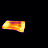
\includegraphics[width=3cm]{images/examples/16494/peas}};
	\node[inner sep=0, label={below:\tiny rapeseed}, below=of b](c){
\includegraphics[width=3cm]{images/examples/16494/rape}};
\end{scope}

\draw (conv) -- (a);
\draw (conv) -- (b);
\draw (conv) -- (c);

%\node[right=2em of b](pred){\includegraphics[width=\classimagewidth]{\prediction}}; %$\hat{\V{y}}$
%
%\draw (a) -- (pred);
%\draw (b) -- (pred);
%\draw (c) -- (pred);

%\draw[endflow] (conv) -- (pred); % node[midway, right] {\small argmax}; 
%\draw[<->] (ground) -- (conv) node[midway, right] {\small $H(\V{y},\hat{\V{y}})$};

\coordinate(cltop) at (concatstates |- labxfw4);

%\node[right=-2em of annotlstm, yshift=0em](lstmcell){\figlstmexplain};

\begin{scope}[on background layer]
	\node[fill=focusone!10, rounded corners, fit=(enczerostatec)(labxfw1)(labxfw4)(rightend), inner sep=.2em]{};
	\node[fill=focustwo!10, rounded corners, fit=(concatstates)(conv)(labct)(cltop), inner sep=.2em]{};
	%\node[fit=(lstmcell)(annotlstm), rounded corners, inner sep=0, noteannot](boxlstm){};
	
\end{scope}


%\node[left=3em of a]{LSTM cell activations:};
\end{tikzpicture}
}
%	\figseqencnetwork
	%\tikzsetnextfilename{network}

\tikzstyle{operator} = [draw, circle, fill=tumbluemedium, draw=tumbluemedium, inner sep=0, text=white]
%\tikzstyle{function} = [draw, rectangle, fill=tumbluemedium, draw=tumbluemedium, text=white]
\tikzstyle{gate} = [fill=tumivory,draw,rounded corners]

\tikzstyle{dummy} = [inner sep=0]
\tikzstyle{flow} = [rounded corners]
\tikzstyle{endflow} = [-stealth,flow]
\tikzstyle{beginflow} = [stealth-,flow]

\tikzstyle{bigpassbox} = [opacity=.2, rounded corners, draw=none]

% defaultvalue -> might be replaced later
\colorlet{tensorcolor}{forwardcolor}

\tikzstyle{bigbox} = [rectangle, draw=tumivory, thick, fill=tumgraylight, rounded corners, 
inner sep=.5ex]

\tikzstyle{wireframe} = [draw=tumgray]
\tikzstyle{image} = [inner sep=0, fill=none, minimum size=\imagewidth]

\tikzset{pic shift/.store in=\shiftcoord,
	pic shift={(0,0)},
	pics/seqlstmfw/.style={
		code={
		\begin{scope}[shift={\shiftcoord},xscale=1.3,yscale=.8]
			
			\node[dummy] (bl) at (0,0){}; % bottom left
			\node[dummy] (tr) at (1,1){}; % top right
			
			\node[dummy] (br) at ($ (bl -| tr) $){}; % bottom right
			\node[dummy] (tl) at ($ (bl |- tr) $){}; % top left
			
			\node[fit=(bl) (tr),bigbox] (-C) {};
			
			% input coordinate for rounded draw lines -> slightly right of tl
			\coordinate (-input) at (0.1,1); % top left
			
			% output coordinate for rounded draw lines -> slightly left of br
			\coordinate (-coutput) at (0.9,0); % bottom right
			\coordinate (-cinput) at (0.1,0); % bottom left
			\coordinate (-houtput) at (0.9,1); % bottom right
			
%			% gate distance
			\def\d{1/6}
			
			% gate heights
			\def\h{1/3}
			
			\coordinate (f)  at bl+(1*\d,0);
			\coordinate (i)  at bl+(2*\d,0);
			\coordinate (j)  at bl+(3*\d,0);
			\coordinate (o)  at bl+(4*\d,0);
			\coordinate (out) at bl+(5*\d,0);
			
			\coordinate (gates) at (0,2*\h);
			
			%\node[above=of tl](xt){$x_{t}$};
			%\node[left=of tl](htminus1){$h_{t-1}$};
			
			%\node[below=of br](ct){$c_{t}$};
			
			\node[gate](fgate) at ($ (gates -| f) $){};
			\node[gate](igate) at ($ (gates -| i) $){};
			\node[gate](jgate) at ($ (gates -| j) $){};
			\node[gate](ogate) at ($ (gates -| o) $){};
			
%			\coordinate (htminus1) at bl+(-.5,0);
%			\coordinate (ht) at bl+(-.5,0);
%			
			% forget gate
			\node[operator](fmult) at ($ (bl -| fgate) $) {};
			\draw[endflow] (-input) -| (fgate) -- (fmult); 
			
%			%j
			\node[operator](jmult) at ([shift={(0,-1*\h)}]jgate) {};
			\node[operator](cadd) at ($ (bl -| jgate) $) {};
			\draw[endflow] (-input) -| (jgate) -- (jmult);
			\draw[endflow] (jmult) -- (cadd); 			

%			%i	
			\draw[endflow] (-input) -| (igate) |- (jmult); 
%
%%			% outpu
			\node[operator](outtanh) at ([shift={(0,1*\h)}]out) {};
%			
%			%o 
			\draw[endflow] (tl) -| (ogate) |- (outtanh);
			\draw[flow] (outtanh) |- (-houtput);
%			
%			% output flow
			\draw[endflow] (cadd) -| (outtanh);
			\draw[flow] (-cinput) -- (fmult) -- (cadd) -- (-coutput);
%			
			
			% debug
%			\node at (gates) {\tiny{gates}};
%			\node at (-input) {\tiny{-input}};
%			\node at (-coutput) {\tiny{-coutput}};
%			\node at (-houtput) {\tiny{-houtput}};
%			\node at (f) {\tiny{f}};
%			\node at (i) {\tiny{i}};
%			\node at (j) {\tiny{j}};
%			\node at (o) {\tiny{o}};
%			\node at (tl) {\tiny{tl}};
%			\node at (br) {\tiny{br}};
%			\node at (bl) {\tiny{bl}};
%			\node at (tr) {\tiny{tr}};
%			\node at (out) {\tiny{out}};
			
		\end{scope}
		}
	}
}

\tikzset{pic shift/.store in=\shiftcoord,
	pic shift={(0,0)},
	pics/seqlstmbw/.style={
		code={
			\begin{scope}[shift={\shiftcoord},xscale=1.3,yscale=-.8]
				
				\node[dummy] (bl) at (0,0){}; % bottom left
				\node[dummy] (tr) at (1,1){}; % top right
				
				\node[dummy] (br) at ($ (bl -| tr) $){}; % bottom right
				\node[dummy] (tl) at ($ (bl |- tr) $){}; % top left
				
				\node[fit=(bl) (tr),bigbox] (-C) {};
				
				% input coordinate for rounded draw lines -> slightly right of tl
				\coordinate (-input) at (0.1,1); % top left
				
				% output coordinate for rounded draw lines -> slightly left of br
				\coordinate (-coutput) at (0.9,0); % bottom right
				\coordinate (-cinput) at (0.1,0); % bottom left
				\coordinate (-houtput) at (0.9,1); % top right
				
				%			% gate distance
				\def\d{1/6}
				
				% gate heights
				\def\h{1/3}
				
				\coordinate (f)  at bl+(1*\d,0);
				\coordinate (i)  at bl+(2*\d,0);
				\coordinate (j)  at bl+(3*\d,0);
				\coordinate (o)  at bl+(4*\d,0);
				\coordinate (out) at bl+(5*\d,0);
				
				\coordinate (gates) at (0,2*\h);
				
				%\node[above=of tl](xt){$x_{t}$};
				%\node[left=of tl](htminus1){$h_{t-1}$};
				
				%\node[below=of br](ct){$c_{t}$};
				
				\node[gate](fgate) at ($ (gates -| f) $){};
				\node[gate](igate) at ($ (gates -| i) $){};
				\node[gate](jgate) at ($ (gates -| j) $){};
				\node[gate](ogate) at ($ (gates -| o) $){};
				
				%			\coordinate (htminus1) at bl+(-.5,0);
				%			\coordinate (ht) at bl+(-.5,0);
				%			
				% forget gate
				\node[operator](fmult) at ($ (bl -| fgate) $) {};
				\draw[endflow] (-input) -| (fgate) -- (fmult); 
				
				%			%j
				\node[operator](jmult) at ([shift={(0,-1*\h)}]jgate) {};
				\node[operator](cadd) at ($ (bl -| jgate) $) {};
				\draw[endflow] (-input) -| (jgate) -- (jmult);
				\draw[endflow] (jmult) -- (cadd); 			
				
				%			%i	
				\draw[endflow] (-input) -| (igate) |- (jmult); 
				%
				%%			% outpu
				\node[operator](outtanh) at ([shift={(0,1*\h)}]out) {};
				%			
				%			%o 
				\draw[endflow] (tl) -| (ogate) |- (outtanh);
				\draw[flow] (outtanh) |- (-houtput);
				%			
				%			% output flow
				\draw[endflow] (cadd) -| (outtanh);
				\draw[flow] (-cinput) -- (fmult) -- (cadd) -- (-coutput);
				%			
				
				% debug
				%			\node at (gates) {\tiny{gates}};
				%			\node at (-input) {\tiny{-input}};
				%			\node at (-coutput) {\tiny{-coutput}};
				%			\node at (-houtput) {\tiny{-houtput}};
				%			\node at (f) {\tiny{f}};
				%			\node at (i) {\tiny{i}};
				%			\node at (j) {\tiny{j}};
				%			\node at (o) {\tiny{o}};
				%			\node at (tl) {\tiny{tl}};
				%			\node at (br) {\tiny{br}};
				%			\node at (bl) {\tiny{bl}};
				%			\node at (tr) {\tiny{tr}};
				%			\node at (out) {\tiny{out}};
				
			\end{scope}
		}
	}
}

\newcommand{\tensorcube}[4]{
	\def\w{#1}
	\def\h{#2}
	\def\d{#3}
%	\def\img{#4}
	
	\begin{scope}[perspective3d]
		
		% bw back frame
		\begin{scope}[canvas is yz plane at x=\d]
			\node[transform shape,image, minimum size=\w, anchor=south west, fill=none, wireframe](back){};
		\end{scope}
		
		% front image
		\begin{scope}[canvas is yz plane at x=0]
			\node[transform shape,image, anchor=south west, opacity=1](front){
				%\includegraphics[width=\w]{\img}
				#4
				};
		\end{scope}
		
		% front frame
		\begin{scope}[canvas is yz plane at x=0]
			\node[transform shape,image, minimum size=\w, anchor=south west, fill=none, wireframe](front){};
		\end{scope}
		
		% fill right side
		\fill[tensorcolor,opacity=.5, wireframe] (front.south east) -- (back.south east) -- (back.north east) -- (front.north east);
		% fill top side
		\fill[tensorcolor,opacity=.5,opacity=0.6, wireframe] (front.north east) -- (back.north east) -- (back.north west) -- (front.north west);
		% fill right side
		
		
		%\draw[] (front.south west) -- (back.south west);
		
	\end{scope}
}

\newcommand{\concatstates}[4]{
	\def\w{#1}
	\def\h{#2}
	\def\d{#3}
	\def\img{#4}
	
	\begin{scope}[perspective3d]
		
		% bw back frame
		\begin{scope}[canvas is yz plane at x=2*\d]
			\node[transform shape,image, minimum size=\w, anchor=south west, fill=none, wireframe](back){};
		\end{scope}
		
		% middle frame
		\begin{scope}[canvas is yz plane at x=\d]
			\node[transform shape,image, minimum size=\w, anchor=south west, fill=none, wireframe](middle){};
		\end{scope}
		
		% front image
		\begin{scope}[canvas is yz plane at x=0]
			\node[transform shape,image, anchor=south west](front){\includegraphics[width=\w]{\img}};
		\end{scope}
		
		% front frame
		\begin{scope}[canvas is yz plane at x=0]
			\node[transform shape,image, minimum size=\w, anchor=south west, fill=none,wireframe](front){};
		\end{scope}
		
		% fill right side
		\fill[backwardcolor,opacity=.5, wireframe] (front.south east) -- (middle.south east) -- (middle.north east) -- (front.north east);
		% fill top side
		\fill[backwardcolor,opacity=.5,opacity=0.6, wireframe] (front.north east) -- (middle.north east) -- (middle.north west) -- (front.north west);
		% fill right side
		
		\fill[forwardcolor,opacity=.5, wireframe] (middle.south east) -- (back.south east) -- (back.north east) -- (middle.north east);
		% fill top side
		\fill[forwardcolor,opacity=.5,opacity=0.6, wireframe] (middle.north east) -- (back.north east) -- (back.north west) -- (middle.north west);
		
		%\draw[] (front.south west) -- (back.south west);
		
		
	\end{scope}
}

\begin{tikzpicture}[scale=1, node distance=1em]%,show background rectangle,background rectangle/.style={draw=red}]

%\matrix (m) [matrix of nodes, ampersand replacement=\&]{

\def\d{1.6}
\def\encoderheight{0.4}
\def\decoderheight{-0.4}
\def\imagewidth{8mm}
\def\stateimagewidth{8mm}
\def\classimagewidth{8mm}

\def\rgbone{images/network/48px/rgb1}
\def\rgbtwo{images/network/48px/rgb2}
\def\rgbthree{images/network/48px/rgb3}
\def\rgbfour{images/network/48px/rgb4}
\def\prediction{images/network/48px/prediction}
\def\groundtruth{images/network/48px/ground_truth}
\def\activation{images/network/48px/maize}
\def\state{images/network/48px/state}


%\draw [bigpassbox, fill=forwardcolor](1,.25) rectangle (10,4);

\node[bigpassbox, fill=forwardcolor, rectangle, minimum width=7cm,minimum height=3cm, anchor=south west, label={[shift={(2em,-3.5ex)}]north:jan $\rightarrow$ dec}] (forwardbox) at (1,.15) {};
%\draw [bigpassbox, fill=backwardcolor](1,-.25) rectangle (10,-4);

\draw pic (fw1) at (\d,\encoderheight) {seqlstmfw};% \&
\node[above=of fw1tl, label=above:{$\VInput_{0}$}](xfw1){\includegraphics[width=\imagewidth]{\rgbone}};%images/network/time1_x

\draw pic (fw2) at (2*\d,\encoderheight) {seqlstmfw};
\node[above=of fw2-input, label=above:{$\VInput_{1}$}](xfw2){\includegraphics[width=\imagewidth]{\rgbtwo}}; % images/network/time11_x

\draw pic (fw3) at (3*\d,\encoderheight) {seqlstmfw};
\node[above=of fw3-input](xfw3){$\dots$};

\draw pic (fw4) at (4*\d,\encoderheight) {seqlstmfw};
\node[above=of fw4-input, label=above:{$\VInput_T$}](xfw4){\includegraphics[width=\imagewidth]{\rgbfour}}; % images/network/time30_x

\node[left=of fw1-input](enczerostateh){$\V{0}$};
\node[left=of fw1-cinput](enczerostatec){$\V{0}$};
\draw[endflow] (enczerostateh) -- (fw1-input);
\draw[endflow] (enczerostatec) -- (fw1-cinput);

% draw connections from input to cells
\draw[flow] (xfw1) |- (fw1-input);
\draw[flow] (xfw2) |- (fw2-input);
\draw[flow] (xfw3) |- (fw3-input);
\draw[flow] (xfw4) |- (fw4-input);

% draw hidden connections between cells
\draw[endflow] (fw1-houtput) -- (fw2-input);
\draw[endflow] (fw2-houtput) -- (fw3-input);
\draw[endflow] (fw3-houtput) -- (fw4-input);

% draw hidden connections between cells
\draw[endflow] (fw1-coutput) -- (fw2-cinput);
\draw[endflow] (fw2-coutput) -- (fw3-cinput);
\draw[endflow] (fw3-coutput) -- (fw4-cinput);

\node[right= 2.5em of fw4-coutput](cfw){$\VCellState_T^\text{fw}$};

\draw[endflow] (fw4-coutput) -- (cfw);

\visible<2->{

\node[bigpassbox, fill=backwardcolor, rectangle, minimum width=7cm,minimum height=3cm, anchor=north west, label={[shift={(2em,3.5ex)}]south:dec $\rightarrow$ jan}] (forwardbox) at (1,-.15) {};

\draw pic (bw1) at (1*\d,\decoderheight) {seqlstmbw};% \&
\node[below=of bw1tl, label=below:{$\VInput_T$}](xbw1){\includegraphics[width=\imagewidth]{\rgbfour}}; % images/network/time30_x

\draw pic (bw2) at (2*\d,\decoderheight) {seqlstmbw};
\node[below=of bw2tl, label=below:{$\VInput_{T-1}$}](xbw2){\includegraphics[width=\imagewidth]{\rgbthree}}; %images/network/time20_x

\draw pic (bw3) at (3*\d,\decoderheight) {seqlstmbw};
\node[below=of bw3tl](xbw3){$\dots$};

\draw pic (bw4) at (4*\d,\decoderheight) {seqlstmbw};
\node[below=of bw4tl, label=below:{$\VInput_0$}](xbw4){\includegraphics[width=\imagewidth]{\rgbone}};

%\node[anchor=center](state) at ($(enc4-coutput)!0.5!(dec1-cinput)$){context state vector $\VCellState_T$};

\node[left=of bw1-input](deczerostateh){$\V{0}$};
\node[left=of bw1-cinput](deczerostatec){$\V{0}$};

\draw[endflow] (deczerostateh) -- (bw1-input);
\draw[endflow] (deczerostatec) -- (bw1-cinput);

% draw state
%\draw[flow] (enc4-coutput) -- ++(.2,0) |- (state);
%\draw[beginflow] (dec1-cinput) -- ++(-.2,0) |- (state);

% draw connections from cells to output
\draw[flow] (xbw1) |- (bw1-input);
\draw[flow] (xbw2) |- (bw2-input);
\draw[flow] (xbw3) |- (bw3-input);
\draw[flow] (xbw4) |- (bw4-input);

\draw[endflow] (bw1-houtput) -- (bw2-input);
\draw[endflow] (bw2-houtput) -- (bw3-input);
\draw[endflow] (bw3-houtput) -- (bw4-input);

\draw[endflow] (bw1-coutput) -- (bw2-cinput);
\draw[endflow] (bw2-coutput) -- (bw3-cinput);
\draw[endflow] (bw3-coutput) -- (bw4-cinput);

\node[right= 2.5em of bw4-coutput](cbw){$\VCellState_T^\text{bw}$};

%\node[right= 6em of fw4-coutput,yshift=.5em, anchor=center,label=left:{$\VCellState^{fw}$}](cfw){
%	%\includegraphics[width=\imagewidth]{images/network/42_state}
%	\begin{tikzpicture}
%	    \colorlet{tensorcolor}{forwardcolor}
%		\tensorcube{\imagewidth}{\imagewidth}{.75}{images/network/42_state}
%	\end{tikzpicture}
%	};
%	
%\node[right= 6em of bw4-coutput, yshift=.5em, anchor=center,label=left:{$\VCellState^{bw}$}](cbw){
%	%\includegraphics[width=\imagewidth]{images/network/72_state}	
%	\begin{tikzpicture}
%	    \colorlet{tensorcolor}{backwardcolor}
%		\tensorcube{\imagewidth}{\imagewidth}{.75}{images/network/72_state}
%	\end{tikzpicture}
%	};

%\draw[endflow] (fw4-coutput) -- +(.25,0);
%\draw[endflow] (bw4-coutput) -- +(.25,0);

\draw[endflow] (bw4-coutput) -- (cbw);

}

\visible<3->{
	
	\node[bigpassbox, fill=classcolor, rectangle, minimum width=5cm,minimum height=3.5cm, anchor=center, label={[shift={(-1ex,-3.5ex)}]north:classification}] (classbox) at (12,0) {};
	
	\node[] (c) at ($(cfw)!0.5!(cbw)$) {};
	
	%\begin{scope}[perspective3d, xshift=10cm]
	%\node[transform shape,image]() at (.5,0,0){\includegraphics[width=\imagewidth]{images/network/72_state}};
	%\node[transform shape,image]() at (.25,0,0){\includegraphics[width=\imagewidth]{images/network/72_state}};
	%\node[transform shape,image]() at (0,0,0){\includegraphics[width=\imagewidth]{images/network/72_state}};
	%\end{scope}
	
	%\node(concatstates) at (6.2*\d,0){
	\node(concatstates) at ($(classbox)+(-1.15cm,0)$){
	\begin{tikzpicture}
	\concatstates{\stateimagewidth}{\stateimagewidth}{1}{\state}
	\end{tikzpicture}
	};
	
	\draw[endflow] (cfw) -- (concatstates);
	\draw[endflow] (cbw) -- (concatstates);
	
	%\path[draw] (0,0) -- (0,1) -- (1,1) -- (1,0) -- (0,0);
	
	\node[right=of concatstates](conv){
		\begin{tikzpicture}
		    \colorlet{tensorcolor}{classcolor}
		    % static
			\tensorcube{\stateimagewidth}{\stateimagewidth}{.75}{\includegraphics[width=\stateimagewidth]{\activation}} %images/network/48px/72_state
	%		\tensorcube{\stateimagewidth}{\stateimagewidth}{.75}{
	%		\animategraphics[poster=16,width=\stateimagewidth,autoplay,loop]{3}{images/network/48px/prediction_scores/prediction_scores-}{0}{16}
	%		}
		\end{tikzpicture}
	};
	
	\node[rectangle, minimum width=4mm, minimum height=4mm, fill=tumgray, draw=tumgray, opacity=.5](inconvrect) at ($ (concatstates) + (-3mm,-3mm) $){};
	%\node[below=0mm of inconvrect](){\tiny \color{white} $\kclass$};
	
	\node[rectangle, minimum width=2mm, minimum height=2mm, fill=tumgray, draw=tumgray, opacity=.5, inner sep=0](outconvrect) at (conv){};
	
	\draw[tumgray] (inconvrect.north east) -- (outconvrect.north west) -- (outconvrect.south west) -- (inconvrect.south east);
	%\draw[tumblack] (inconvrect.north west) -- (outconvrect.north west);
	%\draw[tumblack] (inconvrect.south east) -- (outconvrect.south west);
	%\draw[tumblack] (inconvrect.south west) -- (outconvrect.south west);
	
	\node[below= 3em of conv, label={south:prediction}](pred){\includegraphics[width=\classimagewidth]{\prediction}}; %$\hat{\V{y}}$
	\node[above= 3em of conv, label={north:Ground Truth}](ground){\includegraphics[width=\classimagewidth]{\groundtruth}}; % $\V{y}}$
	
	\draw[endflow] (conv) -- (pred) node[midway, right] {\small $argmax$}; 
	\draw[<->] (ground) -- (conv) node[midway, right] {\small $H(\V{y},\hat{\V{y}})$}; 
}
%};
\end{tikzpicture}

%	
%	%\tikzsetnextfilename{lstm}

\tikzstyle{operator} = [draw, circle, fill=tumbluemedium, draw=tumbluemedium, inner sep=0, text=white]
%\tikzstyle{function} = [draw, rectangle, fill=tumbluemedium, draw=tumbluemedium, text=white]
\tikzstyle{gate} = [] %fill=tumivory,draw,rounded corners=1pt, inner sep=2pt, minimum width=11mm, minimum height=11mm
\tikzstyle{io} = []%fill=tumwhite,draw,rounded corners=1pt, inner sep=2pt, minimum width=11mm, minimum height=11mm

\tikzstyle{dummy} = [inner sep=0]
\tikzstyle{flow} = [rounded corners]
\tikzstyle{endflow} = [-stealth,flow]

\tikzstyle{perspective3drnn}=[
x={(0.5cm,0.5cm)}, y={(1cm,0cm)}, z={(0cm,1cm)}]
\tikzstyle{wireframe} = [draw=tumgray]

\def\image{47-30}

\colorlet{boxcolor}{tumgraylight}
\tikzstyle{bigbox} = [rectangle, draw=tumivory, thick, fill=boxcolor, rounded corners, 
inner xsep=0ex, inner ysep=2ex]

\tikzstyle{annot} = [fill=white, fill opacity=.5, text opacity=1, rounded corners, text=black, xshift=-1.5mm, yshift=-1mm]

\newcommand{\concatstates}[3]{
	\def\w{1cm}%
	\def\h{1cm}%
	\def\d{#1}%
	\def\img{#2}%
	\def\fillcolor{#3}%
	%
	\begin{tikzpicture}[perspective3drnn, rounded corners=0]
		
		% bw back frame
		\begin{scope}[canvas is yz plane at x=2*\d]
			\node[transform shape,inner sep=0, minimum size=\w, anchor=south west, fill=none, wireframe](back){};
		\end{scope}
		
		% front image
		\begin{scope}[canvas is yz plane at x=0]
			\node[inner sep=0, anchor=south west](front){\includegraphics[width=\w]{\img}};
		\end{scope}
		
		% front frame
		\begin{scope}[canvas is yz plane at x=0]
			\node[transform shape,inner sep=0, minimum size=\w, anchor=south west, fill=none,wireframe](front){};
		\end{scope}
		
		\fill[\fillcolor,opacity=.5, wireframe] (front.south east) -- (back.south east) -- (back.north east) -- (front.north east);
		% fill top side
		\fill[\fillcolor,opacity=.5,opacity=0.6, wireframe] (front.north east) -- (back.north east) -- (back.north west) -- (front.north west);
		
	\end{tikzpicture}
}

\tikzset{pic shift/.store in=\shiftcoord,
	pic shift={(0,0)},
	lstmanim/.pic = {
		\begin{scope}[shift={\shiftcoord},xscale=6,yscale=2.5]
			
			\node[dummy] (bl) at (0,0){}; % bottom left
			\node[dummy] (tr) at (1,1){}; % top right
			
			\node[dummy] (br) at ($ (bl -| tr) $){}; % bottom right
			\node[dummy] (tl) at ($ (bl |- tr) $){}; % top left
			
			\node[fit=(bl) (tr),bigbox] (-C) {};
			
			% input coordinate for rounded draw lines -> slightly right of tl
			\coordinate (-input) at (0.1,1); % top left
			
			% output coordinate for rounded draw lines -> slightly left of br
			\coordinate (-coutput) at (0.98,0); % bottom right
			\coordinate (-houtput) at (0.98,1); % bottom right
			
			%			% gate distance
			\def\d{1/5}
			
			% gate heights
			\def\h{1/3}
			
			\coordinate (f)  at bl+(0.7*\d,0);
			\coordinate (i)  at bl+(1.8*\d,0);
			\coordinate (j)  at bl+(2.9*\d,0);
			\coordinate (o)  at bl+(4*\d,0);
			\coordinate (out) at bl+(4.7*\d,0);
			
			\coordinate (gates) at (0,2*\h);
			
			%\node[above=of tl](xt){$x_{t}$};
			%\node[left=of tl](htminus1){$h_{t-1}$};
			
			%\node[below=of br](ct){$c_{t}$};
			
			\node[gate](fgate) at ($ (gates -| f) $){
%				\includegraphics[width=1cm]{images/lstm/f}
				\concatstates{.2}{images/lstm/f}{tumbluelight}
				};
			\node[annot] at (fgate){$\VForgetGate_{t}$};
			
			\node[gate](igate) at ($ (gates -| i) $){
%				\includegraphics[width=1cm]{images/lstm/i}
				\concatstates{.2}{images/lstm/i}{tumbluelight}
				};
			\node[annot] at (igate){$\VInputGate_{t}$};
			
			\node[gate](jgate) at ($ (gates -| j) $){
%				\includegraphics[width=1cm]{images/lstm/j}
				\concatstates{.2}{images/lstm/j}{tumbluelight}
				};
			\node[annot] at (jgate){$\VModulationGate_{t}$};
			
			\node[gate](ogate) at ($ (gates -| o) $){
%				\includegraphics[width=1cm]{images/lstm/o}
				\concatstates{.2}{images/lstm/o}{tumbluelight}
				};
			\node[annot] at (ogate){$\VOutputGate_{t}$};
			
			%			\coordinate (htminus1) at bl+(-.5,0);
			%			\coordinate (ht) at bl+(-.5,0);
			%			
			% forget gate
			\node[operator](fmult) at ($ (bl -| fgate) $) {$ \odot $};
			\draw[flow] (-input) -| (fgate);
			\draw[endflow] (fgate) -- (fmult); 
			
			%			%j
			\node[operator](jmult) at ([shift={(0,-1.3*\h)}]jgate) {$ \odot $};
			\node[operator](cadd) at ($ (bl -| jgate) $) {$ + $};
			\draw[flow] (-input) -| (jgate);
			\draw[endflow] (jgate) -- (jmult);
			\draw[endflow] (jmult) -- (cadd); 			
			
			%			%i	
			\draw[flow] (-input) -| (igate);
			\draw[endflow] (igate) |- (jmult); 
			%
			%%			% outpu
			\node[operator](outtanh) at ($ (jmult -| out) $) {$\odot$};
			%			
			%			%o 
			\draw[flow] (tl) -| (ogate);
			\draw[endflow] (ogate) |- (outtanh);
			\draw[flow] (outtanh) |- (-houtput);
			%			
			%			% output flow
			\draw[endflow] (cadd) -| (outtanh);
			\draw[flow] (fmult) -- (cadd) -- (-coutput);
			%			
			
		\end{scope}
	}
}

\tikzset{pic shift/.store in=\shiftcoord,
	pic shift={(0,0)},
	fgate/.pic = {
		\begin{scope}[shift={\shiftcoord},xscale=1,yscale=1]
			
			\node[dummy] (tl_a) at (0,0){}; % bottom left
			\node[dummy] (br_a) at (1,1){}; % top right
			
			\node[fit=(br_a) (tr_a),gate,inner sep=0] (-C) {};
			
			\node[draw] (conv) at (0.5,0){$conv$}; % bottom left
			\node[draw] (bn) at (0.5,.5){$bn$}; % bottom left
			\node[draw] (sigmoid) at (0.5,1){$\sigma$}; % bottom left
				
		\end{scope}
	}
}

\newcommand{\grutwo}{
\begin{tikzpicture}[scale=1, node distance=2em]%,show background rectangle,background rectangle/.style={draw=red}]
\draw pic (GRU) at (0,0) {gru};
\node[io,left=of GRU-hinput](gru_htminus1){$\VHidden_{t-1}$};
\draw[rounded corners] (gru_htminus1) -| (GRU-hinputflow);
\node[io,above=of GRU-xinput](gru_xt){$\VInput_{t}$};

\draw[rounded corners] (gru_xt) |- (GRU-xinputflow);

\node[io,right=of GRU-houtput](gru_ht){$\VHidden_{t}$};
\draw[rounded corners] (GRU-houtput)--(gru_ht);
\end{tikzpicture}
}

\newcommand{\lstmanimtwo}{
	\begin{tikzpicture}[scale=1, node distance=1em]%,show background rectangle,background rectangle/.style={draw=red}]
	
	
	\draw pic (LSTM) at (0,0) {lstmanim};
	\node[io,left=of LSTMtl](htminus1){
%		\includegraphics[width=1cm]{images/lstm/o}
		\concatstates{.2}{images/lstm/h_}{tumblue}
	};
	\node[annot] at (htminus1){$\VHidden_{t-1}$};

	\draw[endflow] (htminus1) -- (LSTM-input);
	\node[io,right=of LSTMbr](ct){%
%		\includegraphics[width=1cm]{images/lstm/c}
		\concatstates{.2}{images/lstm/c}{tumblue}
	}; % $c_{t}$
	\node[annot] at (ct){$\VCellState_{t}$};

	\draw[endflow] (LSTM-coutput)--(ct);
	\node[io,left=of LSTMbl](ctminus1){%
		%\includegraphics[width=1cm]{images/lstm/c}
		\concatstates{.2}{images/lstm/c_}{tumblue}
	}; % 
	\node[annot] at (ctminus1){$\VCellState_{t-1}$};

	\draw[endflow] (ctminus1)--(LSTMfmult);
	\node[io,right=of LSTMtr](ht){
		%\includegraphics[width=1cm]{images/lstm/h}
		\concatstates{.2}{images/lstm/h}{tumblue}
	};
	\node[annot] at (ht){$\VHidden_{t}$};

	\draw[endflow] (LSTM-houtput)--(ht);
	
    \draw[endflow] (ct) -- ($ (ct)+(0,-1) $) -| (ctminus1);
	\draw[endflow] (ht) -- ($ (ht)+(0,1) $) -| (htminus1);
	
    \node[io,xshift=1ex,above=2em of LSTMtl,label=left:$\VInput_{t}$](xt){%
		%\includegraphics[width=1cm]{images/lstm/x}
		\concatstates{.1}{images/lstm/x}{tumorange}
	};%$x_{t}$

	\draw[rounded corners] (xt) |- (LSTM-input);
	

	\node[right=of ct, yshift=0em ](concatstates){
%		\begin{tikzpicture}
		\concatstates{.2}{images/lstm/cT}{tumblue}
%		\end{tikzpicture}
	};

	\node[right=of concatstates](conv){
		\concatstates{.1}{images/examples/16494/rape}{tumblue}
	};

	\coordinate (center) at ($ (concatstates) + (1mm,-3mm) $);

	\node[rectangle, minimum width=4mm, minimum height=4mm, fill=tumblue, draw=tumblue, opacity=.5, rounded corners=0, semithick](inconvrect) at (center){};
	
	\node[rectangle, minimum width=2mm, minimum height=2mm, fill=tumblue, draw=tumblue, opacity=.5, inner sep=0, semithick, rounded corners=0, xshift=2mm, yshift=-2.5mm](outconvrect) at (conv){};
	
	\draw[tumblue, semithick, rounded corners=0, fill=tumbluedark, opacity=.2] (inconvrect.north east) -- (outconvrect.north west) -- (outconvrect.south west) -- (inconvrect.south east);
	
	
	\begin{scope}[node distance=.5em]
	\node[inner sep=0, label={below:\tiny class A}, above= 2em of concatstates, xshift=0](a){\includegraphics[width=1cm]{images/examples/16494/maize}};
	\node[inner sep=0, label={below:\tiny class B}, right=of a](b){\includegraphics[width=1cm]{images/examples/16494/meadow}};
	\node[inner sep=0, label={below:\tiny class C}, right=of b](c){\includegraphics[width=1cm]{images/examples/16494/peas}};
%	\node[inner sep=0, label={below:\tiny peas}, right=of c](d){\includegraphics[width=1cm]{images/examples/16494/peas}};
%	\node[inner sep=0, label={below:\tiny rapeseed}, right=of d](e){\includegraphics[width=1cm]{images/examples/16494/rape}};
	\end{scope}
	
	\node[fit=(a)(b)(c), draw=tumgray, inner sep=1em, rounded corners, label={above:predictions}](predictions){};
	
	\draw[endflow, draw=tumgray] (conv) -- (predictions);
	
	\draw[endflow] (ct) -- node[midway, above]{$\VCellState_{T}$} (concatstates);
	
	
	\end{tikzpicture}
}
%	\lstmanimtwo
t\end{frame}

\begin{frame}
\frametitle{It worked very well}
% \begin{tabular}{@{}
%                 V{26mm}
%                 v{10mm}
%                 v{28mm}
%                 v{20mm}
%                 v{15mm}
%                 v{10mm}
%                 p{10mm}
%                 @{}}
%   1 & 2 & 3 & 4 & 5 & 6 & 7 \\
%   1 & 2 & 3 & 4 & 5 & 6 & 7
% \end{tabular}
% \def\cellwidth{2cm}
% short alias for multocol
%{\Large %  
% \renewcommand{\arraystretch}{1.3}
% atmospheric correction
\newcommand{\atcor}{atmospheric correction}

%\begin{tabularx}{\textwidth}{p{3cm}|p{.8cm}p{.5cm}p{.3cm}XXXXX}
% \begin{tabularx}{\textwidth}{
% 		p{2.6cm} 	% approach
% 		p{.75cm}| 	% year
% 		p{1cm}    	% sensor
% 		p{2.8cm}		% preprocessing
% 		p{2cm}		% features
% 		p{1.3cm}	% classifier
% 		p{1cm}		% accuracy
% 		p{1cm}		% classes
% 		}
\begin{tabular}{@{}
                X
                x
                x
                x
                @{}}
\toprule
% \multicolumn{1}{X}{Year} & 
%\multicolumn{3}{p{2.4cm}}{Data}&
\multicolumn{1}{X}{Approach} &
\multicolumn{1}{X}{Preprocessing} &
\multicolumn{1}{X}{Accuracy} &
\multicolumn{1}{X@{}}{\# Classes} \\ 

\cmidrule(r){1-1}
\cmidrule(lr){2-2}
\cmidrule(lr){3-3}
\cmidrule(lr){4-4}
\addlinespace
% %                        
% %& Sensor& 
% %Objects& 
% %\scriptsize Cl. &  
% %&        
% %&          
% %\\ 
% %  
% % \hline
% %% this approach 18
\textbf{Rußwurm \& Körner (2018)} & 
% 2018 &
%7.7m \scriptsize $px^{10m}$ & 
\textbf{none} &  
\textbf{90} &
17 \\
\addlinespace
% 1 & 2 & 3 & 4 & 5 & 6  \\
% 1 & 2 & 3 & 4 & 5 & 6  \\
% % % 
%% \citet{Russwurm17:TVM}
Rußwurm \& Körner (2017) & 

%500k \scriptsize $px^{30m}$ & 
\atcor&
74 & % \footnote{excluding covered classes}
\textbf{18} \\ 
\addlinespace
% % 
% % %% Siachalou15
{Siachalou et a. (2015)} & 
% 2015 &
%3k {\scriptsize parcels} & 
geometric correction,
image registration & 
\textbf{90} & % 89.7 from their abstract
6 \\ 
\addlinespace
% % 
% % %% Hao15
Hao et al. (2015) &
% 2015 &
%6k \scriptsize $px^{500m}$ &  
image reprojection, \atcor &
89 &
6 \\ 
\addlinespace
% % 
% % %% Conrad14
Conrad et al. (2014) &
% 2014 &
%423 {\scriptsize parcels} &  
segmentation, \atcor &
86 &
9 \\ 
\addlinespace
% % 
% % %% Foerster
Förster et al. (2012) &
% 2012 
%18k \scriptsize $px^{30m}$ &  
phen. normalization, \atcor &
73 &
11 \\ 
\addlinespace
% % 
% % %% Barragan11
Barragan et al. (2011) &
% 2011 &
%650 {\scriptsize parcels} &  
segmentation, \atcor &
79 &
13 \\ 
\addlinespace
% % 
% % 
% % 
% % %% Conrad10
% 2010 &
Conrad et al. (2010) & 
%$196$ {\scriptsize parcels} &  
segmentation, \atcor &
80 &
6 \\ 
% % 
\addlinespace
\bottomrule
% %	
% %Approach               & Features   & Classifier & Sensor                                    & Region    & Class obj \\ 
% %this approach          & TOA refl   & ConvRNN    & {s2} & 7.7 mio $px^{10m}$\\ 
% %\citet{Russwurm17:TVM} & BOA refl   & RNN        & {s2} & 500k $patch^{30m}$\\ 
% %\citet{Foerster2012}   & NDVI stat  & DT         & {ls} & 18k $px^{30m}$\\ 
% %\citet{Hao15}          & NDVI stats + TOA refl.  & RF & {modis} & 6k $px^{500m}$ \\ 
% %\citet{conrad2010}     & Veg Ind.   & OBIA+DT    & {spot}\newline{aster} & 196 parcels \\ 
% %\citet{conrad2014}     & Veg Ind.   & OBIA+RF    & {spot}, {rapideye}, {quickbird} & 423 parcels  \\ % table2 -> 47+81+47+47+72+34+25+39+31
% %%\citet{Jakubauskas2002}& NDVI harm. & discr. anal& \satellite{Avhrr}                         & Kansas, USA&&\\ 
% %\citet{Barragan2011}   & Veg Ind.   & OBIA+DT    & {aster} & 650 parcels\\ 
% %\citet{Siachalou2015}  & TOA refl.  & OBIA+HMM   & {ls}, {rapideye} & 3k parcels\\ 
% %
% %\\
% %\hline
% %\\
% %
% %
% %approach               & n classes & overall accuracy & prod. selection\\ 
% %this approach          & 18        &                  & autom. filter <80\% cl \\ 
% %\citet{Russwurm17:TVM} & 18        & 74.3             & autom. filter <80\% cl \\ 
% %\citet{Foerster2012}   & 11        & 72.8             & man. cloudfree sel. \\ 
% %\citet{Hao15}          & 6         & 88.8             & \satellite{eModis}/\satellite{Modis} align. \newline + man. cloudfree sel.\\ 
% %\citet{conrad2010}     & 6         & 80.1             & man. cloudfree sel. \\ 
% %\citet{conrad2014}     & 9         & 85.7             & man. cloudfree sel. \\ 
% %%\citet{Jakubauskas2002}& 6         & 51.7             &       & \\ % from 2002
% %\citet{Barragan2011}   & 13        & 79               & based on crop cal. + \newline man. cloudfree sel. \\
% %\citet{Siachalou2015}  & 6         & 92.5             & man. cloudfree sel. \\ 
% %
% %\\
% %\hline
% %\\
% %
% %% image cost: none if all satellites free; medium is combination of free and commercial and high if all satellites commercial
% %
% %approach                & atm. corr.           & preproc.                & expert knowledge \\ 
% %this approach           & no                   & img. cropping                    &                  \\ 
% %\citet{Russwurm17:TVM}  & yes (\brand{sen2cor})& img. cropping/interp.            &                  \\ 
% %\citet{Foerster2012}    & yes \cite{Richter1996})  & VI calc.                & agro-meteor info \\ 
% %\citet{Hao15}           &                      & CRS reproj/ VI calc     &                  \\ 
% %\citet{conrad2010}      & yes \cite{Richter1996})  & obj. segm./ VI calc     & class. rules     \\ 
% %\citet{conrad2014}      & yes \cite{Richter1996})  & obj. segm./ VI calc     &                  \\ 
% %\citet{Barragan2011}    & yes \cite{Matthew2000}) & obj. segm./ VI calc& expert consultation \\ 
% %\citet{Siachalou2015}   & no                   & image reg./ pansharp./ resampl. &          \\ 
% %	
% %% flaash tool  Matthew et al., 2000 ) with local atmosphere and aerosol content                   
% %	
\end{tabular}       

\end{frame}

%\newcommand{\examplescenescbar}{
	\begin{tikzpicture}[inner sep=0]
	\node(cbar){\includegraphics[height=\size, width=2mm]{images/examples/inferno}};
	\node[xshift=1mm, anchor=north] at (cbar.north east){\tiny 1};
	\node[xshift=1mm, anchor=south] at (cbar.south east){\tiny 0};
	\end{tikzpicture}
}


% for text extending below like p, q, g
%\tikzset{
%	mylabel2/.style={
%		label={
%			[label distance=-1.25em, anchor=base]north:
%			\fcolorbox{black}{black}{
%				\scriptsize \color{tumgraylight} #1
%			}
%		}
%	}
%}

\newcommand{\tileexample}[9]{
\\ %% good classificaiton example
\node[inner sep=0]{\includegraphics[width=\size]{images/examples/#1/rgb}}; \&
\node[inner sep=0]{\includegraphics[width=\size]{images/examples/#1/ground_truth}}; \&
\node[inner sep=0]{\includegraphics[width=\size]{images/examples/#1/prediction}}; \&
\node[inner sep=0]{\includegraphics[width=\size]{images/examples/#1/masked_loss}}; \&
\node[inlabel=#3,inner sep=0]{\includegraphics[width=\size]{images/examples/#1/#2}}; \&
\node[inlabel=#5,inner sep=0]{\includegraphics[width=\size]{images/examples/#1/#4}}; \&
\node[inlabel=#7,inner sep=0]{\includegraphics[width=\size]{images/examples/#1/#6}}; \&
\node[inlabel=#9,inner sep=0]{\includegraphics[width=\size]{images/examples/#1/#8}}; \&
\examplescenescbar 	
}

%\\ %% good classificaiton example
%\node[rowlabel=A,inner sep=0]{\includegraphics[width=\size]{images/examples/16494/rgb}}; \&
%\node[inner sep=0]{\includegraphics[width=\size]{images/examples/16494/ground_truth}}; \&
%\node[inner sep=0]{\includegraphics[width=\size]{images/examples/16494/prediction}}; \&
%\node[inner sep=0]{\includegraphics[width=\size]{images/examples/16494/masked_loss}}; \&
%\node[inlabel=maize,inner sep=0]{\includegraphics[width=\size]{images/examples/16494/maize}}; \&
%\node[inlabel=meadow,inner sep=0]{\includegraphics[width=\size]{images/examples/16494/meadow}}; \&
%\node[inlabel=peas,inner sep=0]{\includegraphics[width=\size]{images/examples/16494/peas}}; \&
%\node[inlabel=rape,inner sep=0]{\includegraphics[width=\size]{images/examples/16494/rape}}; \&
%\examplescenescbar 	

\newcommand{\makeexamplelegend}{
\tiny
%\node[inner sep=0]{\includegraphics[width=\size]{images/examples/color__asparagus}};
\matrix (n) [matrix of nodes, ampersand replacement=\&, row sep=0pt, column sep=2mm, below= 0mmof m]{
	\node[collabel=aspar., inner sep=0]{\includegraphics[width=\colsize]{images/examples/color__asparagus}}; \&
	\node[collabel=bean,inner sep=0]{\includegraphics[width=\colsize]{images/examples/color__beans}}; \&
	\node[collabel=hop,inner sep=0]{\includegraphics[width=\colsize]{images/examples/color__hop}}; \&
	\node[collabel=maize,inner sep=0]{\includegraphics[width=\colsize]{images/examples/color__maize}}; \&
	\node[collabel=mead.,inner sep=0]{\includegraphics[width=\colsize]{images/examples/color__meadow}}; \&
	\node[collabel=peas,inner sep=0]{\includegraphics[width=\colsize]{images/examples/color__peas}}; \&
	\node[collabel=pot.,inner sep=0]{\includegraphics[width=\colsize]{images/examples/color__potatoe}}; \&
	\node[collabel=rape,inner sep=0]{\includegraphics[width=\colsize]{images/examples/color__rape}}; \&
	\node[collabel=soyb.,inner sep=0]{\includegraphics[width=\colsize]{images/examples/color__soybeans}}; \&
	\node[collabel=beet,inner sep=0]{\includegraphics[width=\colsize]{images/examples/color__sugar_beet}}; \&
	\node[collabel=s.barl,inner sep=0]{\includegraphics[width=\colsize]{images/examples/color__summer_barley}}; \&
	\node[collabel=oat,inner sep=0]{\includegraphics[width=\colsize]{images/examples/color__summer_oat}}; \&
	\node[collabel=w.barl,inner sep=0]{\includegraphics[width=\colsize]{images/examples/color__winter_barley}}; \&
	\node[collabel=rye,inner sep=0]{\includegraphics[width=\colsize]{images/examples/color__winter_rye}}; \&
	\node[collabel=spelt,inner sep=0]{\includegraphics[width=\colsize]{images/examples/color__winter_spelt}}; \&
	\node[collabel=tritic,inner sep=0]{\includegraphics[width=\colsize]{images/examples/color__winter_triticale}}; \&
	\node[collabel=wheat,inner sep=0]{\includegraphics[width=\colsize]{images/examples/color__winter_wheat}}; \&
	\\
};	
	
}

\tikzset{
	collabel/.style={
		label={
			[label distance=1.5em, anchor=base]south:
			\scriptsize \color{black} #1
		}
	}
}

\setlength{\fboxsep}{1pt}
\tikzset{
	inlabel/.style={
		label={
			[label distance=-1em, anchor=base]north:
			\fcolorbox{black}{black}{
				\scriptsize \color{tumgraylight} #1
			}
		}
	}
}

\tikzset{
	rowlabel/.style={
		label={
			[label distance=.51em, anchor=north west]north west:
			\fcolorbox{white}{white}{
				\color{black} \textbf{ \scriptsize #1 }
			}
		}
	}
}

\def\size{1.4cm}
\def\colsize{5mm}

%\colsize
\small

\newcommand{\makeimage}{

\begin{tikzpicture}

\matrix (m) [matrix of nodes, ampersand replacement=\&, row sep=0pt, column sep=2mm]{
	$\V{x}_{RGB,t}$ \& labels $\V{y}$ \& pred. $\hat{\V{y}}$ \& loss $H(\V{y},\hat{\V{y}}$) \& activation \& activation \& activation \& activation
	\tileexample{16494}{maize}{maize}{meadow}{meadow}{peas}{peas}{rape}{rape}
%	\\ %% Good example with correct prediction, but some loss
	\tileexample{8133}{winter_spelt}{spelt}{winter_wheat}{wheat}{summer_barley}{s.barley}{maize}{maize}
%	\\ %% Good example, only one small field partly wrong classified
	\tileexample{1823}{meadow}{meadow}{winter_wheat}{wheat}{summer_oat}{oat}{maize}{maize}
	\\ %% narrow fields
	\tileexample{12894}{meadow}{meadow}{winter_wheat}{wheat}{potatoe}{potato}{maize}{maize}
	\tileexample{2550}{maize}{maize}{winter_wheat}{wheat}{summer_barley}{s.barley}{winter_barley}{w.barley}
%	\\ %% Good example, only one small field partly wrong classified
	\tileexample{2554}{maize}{maize}{winter_wheat}{wheat}{meadow}{meadow}{winter_barley}{w.barley}
%	\\ %% Exampe of a forrest, which us a unknown class!
	\tileexample{10791}{maize}{maize}{winter_wheat}{wheat}{meadow}{meadow}{winter_barley}{w.barley}
%	\\ %% sparse label feature map
	\tileexample{10792}{winter_rye}{rye}{winter_wheat}{wheat}{winter_triticale}{triticale}{summer_barley}{s.barley}
%	\\ %% one field completely wrong classified. one field uncertain
	\tileexample{10879}{winter_rye}{rye}{winter_triticale}{triticale}{summer_barley}{s.barley}{winter_barley}{w.barley}
%	\\ %% Multiple fields uncertain
	\tileexample{10969}{winter_wheat}{wheat}{winter_triticale}{triticale}{winter_rye}{rye}{rape}{rape}
	%% one field uncertain
	\tileexample{172}{winter_wheat}{wheat}{meadow}{meadow}{maize}{maize}{winter_barley}{w.barley}
	\\
};

\makeexamplelegend
\end{tikzpicture}

}
%\begin{frame}
%\frametitle{Qualitative Examples}
%%	\framesubtitle{ConvGRU with r=256 recurrent cells}
%\centering
%\begin{tikzpicture}
%\matrix (m) [matrix of nodes, ampersand replacement=\&, row sep=0pt, column sep=2mm]{
%	$\V{x}_{RGB,t}$ \& labels $\V{y}$ \& pred. $\hat{\V{y}}$ \& $H(\V{y},\hat{\V{y}}$) \& activation \& activation \& activation \& activation
%	\tileexample{16494}{maize}{maize}{meadow}{meadow}{peas}{peas}{rape}{rape}
%	\tileexample{8133}{winter_spelt}{spelt}{winter_wheat}{wheat}{summer_barley}{s.barley}{maize}{maize}
%	\tileexample{12894}{meadow}{meadow}{winter_wheat}{wheat}{potatoe}{potato}{maize}{maize}
%	%		\tileexample{1823}{meadow}{meadow}{winter_wheat}{wheat}{summer_oat}{oat}{maize}{maize}
%	\\
%};
%\makeexamplelegend
%\end{tikzpicture}
%\end{frame}

%\begin{frame}
%\frametitle{Qualitative Examples}
%%	\framesubtitle{ConvGRU with r=256 recurrent cells}
%\centering
%\begin{tikzpicture}
%\matrix (m) [matrix of nodes, ampersand replacement=\&, row sep=0pt, column sep=2mm]{
%$\V{x}_{RGB,t}$ \& labels $\V{y}$ \& pred. $\hat{\V{y}}$ \& $H(\V{y},\hat{\V{y}}$) \& activation \& activation \& activation \& activation
%\tileexample{10879}{winter_rye}{rye}{winter_triticale}{triticale}{summer_barley}{s.barley}{winter_barley}{w.barley}
%\tileexample{10792}{winter_rye}{rye}{winter_wheat}{wheat}{winter_triticale}{triticale}{summer_barley}{s.barley}
%%		\tileexample{10969}{winter_wheat}{wheat}{winter_triticale}{triticale}{winter_rye}{rye}{rape}{rape}
%\tileexample{172}{winter_wheat}{wheat}{meadow}{meadow}{maize}{maize}{winter_barley}{w.barley}
%\\
%};
%\makeexamplelegend
%\end{tikzpicture}
%\end{frame}


%\begin{frame}
%\frametitle{How did the ConvRNN handle the cloud noise?}
%
%We performed two experiments
%\begin{enumerate}
%	\item Visualization of internal network states. We found some hidden states that were sensitive 
%\end{enumerate}
%
%\end{frame}

\begin{frame}
\LARGE
\centering
\textbf{How did the ConvLSTM handle the clouds?}
\end{frame}


\begin{frame}
\frametitle{Experiments}
\LARGE
1. \textbf{Visualization of hidden states}

{\hspace{2em} we found specific states dedicated for cloud masking.}

\vspace{2em}
2. \textbf{Ablation experiment on different cloud coverages} 

{\hspace{2em} similar accuracies on different degrees of cloud coverage.}

\end{frame}

\begin{frame}
	\frametitle{Takeaways \& Poster}
	
	\LARGE
	1. \textbf{ConvRNNs were very robust when considering noisy data}
	
	\vspace{2em}
	2. \textbf{Would love to hear other's experiences on this}
	
\end{frame}

%\begin{frame}
%\frametitle{Looking back at the Unreasonable Effectiveness of RNNs Blog}
%\texttt{http://karpathy.github.io/2015/05/21/rnn-effectiveness/}
%\includegraphics[width=\textwidth]{images/karpathy_charrnn}
%\end{frame}

%\newcounter{tcounter}

\newcommand{\drawcbar}[5]{
	\def\tnode{#1} % iGate0
	\def\cmap{#2} % inferno
	\def\cbarheight{#3} % 1cm
	%	\def\vmin{#4} % 0
	%	\def\vmax{#5} % 1
	
	\node[xshift=1mm] (cbar\tnode) at (\tnode.east){\includegraphics[height=2mm, width=\cbarheight, angle=90,origin=c]{\cmap}};
	\node[anchor=south] at (cbar\tnode.south east) {\tiny #4};
	\node[anchor=north] at (cbar\tnode.north east) {\tiny #5};
}
\newcommand{\imagecolumns}[2]{
		\foreach \t in {#1,...,#2}{
			\node(times) at (\thetcounter*\hdist,0*\vdist){$t_{\the\numexpr\t+1\relax}$};
			\node[activation](xlast) at (\thetcounter*\hdist,-1*\vdist){\includegraphics[width=\imagewidth]{\folder/sample\s/time\t_x}};
			
			\node[activation, yshift=-1mm](flast1) at (\thetcounter*\hdist,-2*\vdist){\includegraphics[width=\imagewidth]{\folder/sample\s/time\t/\done_fGate}};
			\node[activation, yshift=-1mm](ilast1) at (\thetcounter*\hdist,-3*\vdist){\includegraphics[width=\imagewidth]{\folder/sample\s/time\t/\done_iGate}};
			\node[activation, yshift=-1mm](jlast1) at (\thetcounter*\hdist,-4*\vdist){\includegraphics[width=\imagewidth]{\folder/sample\s/time\t/\done_jGate}};
			\node[activation, yshift=-1mm](clast1) at (\thetcounter*\hdist,-5*\vdist){\includegraphics[width=\imagewidth]{\folder/sample\s/time\t/\done_state}};
			
			\stepcounter{tcounter}
		}
	}
	
\newcommand{\dotscolumn}{
	\node[activation] at (\thetcounter*\hdist,-1*\vdist){$\dots$};
	
	\node[activation,yshift=-1mm] at (\thetcounter*\hdist,-2*\vdist){$\dots$};
	\node[activation,yshift=-1mm] at (\thetcounter*\hdist,-3*\vdist){$\dots$};
	\node[activation,yshift=-1mm] at (\thetcounter*\hdist,-4*\vdist){$\dots$};
	\node[activation,yshift=-1mm] at (\thetcounter*\hdist,-5*\vdist){$\dots$};
	\stepcounter{tcounter}
	}

\newcommand{\figactivations}[2]{
	% 1: number of sample
	% 2. number of activation
	
	\setcounter{tcounter}{0}
	
	\begin{tikzpicture}
	%\figGates{0}{18}{1}{3}
	\def\folder{images/activations/48px}
	
	\tikzstyle{activation}=[]
	\def\s{#1}
	
	\def\done{#2}
%	\def\dtwo{22}
%	\def\dthree{47}
	
	%% grid distance vertical and horizontal
	\def\vdist{8.5mm}
	\def\hdist{8.5mm}
	
	\def\imagewidth{8mm}
	
	
	%% descriptions top row
	\node[anchor=west] at (-1.5*\hdist,-1*\vdist){$\V{x}$};
	\node[anchor=west, yshift=-1mm](f1) at (-1.5*\hdist,-2*\vdist){$\V{f}^{(\done)}$};
	\node[anchor=west, yshift=-1mm](i1) at (-1.5*\hdist,-3*\vdist){$\V{i}^{(\done)}$};
	\node[anchor=west, yshift=-1mm](j1) at (-1.5*\hdist,-4*\vdist){$\V{j}^{(\done)}$};
	\node[anchor=west, yshift=-1mm](c1) at (-1.5*\hdist,-5*\vdist){$\V{c}^{(\done)}$};


	\imagecolumns{0}{1}
	\dotscolumn
	\imagecolumns{9}{14}
	\dotscolumn
	\imagecolumns{30}{34}
	
	
	\drawcbar{flast1}{images/activations/inferno}{\imagewidth}{0}{1}
	\drawcbar{ilast1}{images/activations/inferno}{\imagewidth}{0}{1}
	\drawcbar{jlast1}{images/activations/RdBu_r}{\imagewidth}{-1}{1}
	\drawcbar{clast1}{images/activations/RdBu_r}{\imagewidth}{-1}{1}
	
	
	
	\end{tikzpicture}
}
%\begin{frame}
%\frametitle{Cloud Sensitive Cells}
%\framesubtitle{LSTM cell \textbf{47} of 256}
%\figactivations{1}{47}
%\end{frame}
%
%\begin{frame}
%\frametitle{Ablation Experiment on Cloudy Data}
%%usepgfplotslibrary{fillbetween}

%\newcommand{\fbopacity}{0.3}
%\newcommand{\skippoints}{2}


%\def\measure{oa}
\def\height{3.5cm}


%\colorlet{L1Ccolor}{tumblue}
%colorlet{L2Acolor}{tumblack}

%\colorlet{clouds01color}{tumred}
%\colorlet{clouds10color}{tumorange}
%\colorlet{clouds25color}{tumgray}
%\colorlet{clouds50color}{tumblue}
%\colorlet{clouds80color}{tumblack}

\colorlet{clouds01color}{tumbluedark!55}
\colorlet{clouds10color}{tumbluedark!70}
\colorlet{clouds25color}{tumbluedark!85}
\colorlet{clouds50color}{tumbluedark}
\colorlet{clouds80color}{tumblack}

\colorlet{highlightcolor}{tumgraylight!25}

%\colorlet{2017traincolor}{tumgray}
%\colorlet{2017testcolor}{tumblack}

\tikzset{new spy style/.style={spy scope={%
			magnification=2,
			connect spies,
			every spy on node/.style={
				rectangle,
				rounded corners=1pt,
				draw,
			},
			every spy in node/.style={
				draw,
				rectangle,
				rounded corners=1pt,
				fill=gray!40,
			}
		}
	}
} 


\tikzsetnextfilename{clouds}
\begin{tikzpicture}[new spy style, remember picture]
	
	% replaced by global settings in figures.tex
%	\pgfplotsset{every axis plot/.append style={line width=1pt}}
	
	
	\begin{groupplot}[
	group style={
		group size=2 by 1,
		xlabels at=edge bottom,
		ylabels at=edge left,
		xticklabels at=edge bottom,
		vertical sep=35pt,
		group name=trainplot
	},
	legend style={
		at={(1.65,0)},
		anchor=south,
		fill=tumgraylight!50,
		rounded corners=1pt,
		draw=none,
		font=\scriptsize, 
		legend image post style={line width =3pt},
		/tikz/every even column/.append style={column sep=0.2cm},
	},
	axis lines=left,
	grid=both,
	scaled x ticks = false,
	y tick label style={/pgf/number format/fixed},
	grid style={draw=tumgraylight},
	legend columns=1,
	width=.38\textwidth,
	height=\height,
	xlabel={samples seen},
	xmin=-10000,
	xmax=800000,
	ymin=.85,
	ymax=.95]


\nextgroupplot[title=,ylabel={ov. acc.},ymin=.2,ymax=1]


\coordinate (topsource) at (axis cs: 800000,.96);
\coordinate (bottomsource) at (axis cs: 800000,.84);

\coordinate (topsourceleft) at (axis cs: 0,.96);
\coordinate (bottomsourceleft) at (axis cs: 0,.84);

\fill[highlightcolor,draw=tumgraylight, rounded corners=1pt] (bottomsource) -- (bottomsourceleft) -- (topsourceleft) -- (topsource); 

\addplot[clouds01color, forget plot] table [x=Step, y = clouds01_test2016clouds01_oa, col sep=comma] {images/clouds/train_rw3.csv};

\addplot[clouds10color, forget plot] table [x=Step, y = clouds10_test2016clouds10_oa, col sep=comma] {images/clouds/train_rw3.csv};

\addplot[clouds25color, forget plot] table [x=Step, y = clouds25_test2016clouds25_oa, col sep=comma] {images/clouds/train_rw3.csv};

\addplot[clouds50color, forget plot] table [x=Step, y = clouds50_test2016clouds50_oa, col sep=comma] {images/clouds/train_rw3.csv};

\addplot[clouds80color, forget plot] table [x=Step, y = clouds80_test2016_oa, col sep=comma] {images/clouds/train_rw3.csv};

\nextgroupplot[
	title=,
	ylabel={ov. acc.}, 
	ymin=.84,
	ymax=.96, 
	xmin=0,
	axis y line*=right,
	ylabel near ticks, 
	yticklabel pos=right,
	grid=both,
	grid style={tumgray!50},
	axis background/.style={fill=highlightcolor},
	]
\addplot[clouds01color] table [x=Step, y = clouds01_test2016clouds01_oa, col sep=comma] {images/clouds/train_rw15.csv};
\addlegendentry{$<$ \SI{1}{\percent} (4 obs.)}

\addplot[clouds10color] table [x=Step, y = clouds10_test2016clouds10_oa, col sep=comma] {images/clouds/train_rw15.csv};
\addlegendentry{$<$ \SI{10}{\percent} (10 obs.)}

\addplot[clouds25color] table [x=Step, y = clouds25_test2016clouds25_oa, col sep=comma] {images/clouds/train_rw15.csv};
\addlegendentry{$<$ \SI{25}{\percent} (17 obs.)}

\addplot[clouds50color] table [x=Step, y = clouds50_test2016clouds50_oa, col sep=comma] {images/clouds/train_rw15.csv};
\addlegendentry{$<$ \SI{50}{\percent} (23 obs.)}

\addplot[clouds80color] table [x=Step, y = clouds80_test2016_oa, col sep=comma] {images/clouds/train_rw15.csv};
\addlegendentry{all images (46 obs.)}

\coordinate (toptarget) at (rel axis cs: 0,1);
\coordinate (bottomtarget) at (rel axis cs: 0,0);

\end{groupplot}

\draw[fill=highlightcolor, draw=tumgraylight] (topsource) -- (toptarget) -- (bottomtarget)  -- (bottomsource);
\draw[|-|, tumgray] ($ (bottomsource) + (0ex,0) $) -- ($ (topsource) + (0ex,0) $);
\draw[|-|, tumgray] (bottomtarget) -- (toptarget);

\end{tikzpicture}  

%\end{frame}

\begin{frame}[c]
\frametitle{Publications and Code}
\centering 

\Large



Github + DockerHub

\vspace{1ex}

\includegraphics[width=2cm]{images/github} \hspace{.5ex}
\includegraphics[width=2cm]{images/qr_github} \hspace{.5ex}
\includegraphics[width=2cm]{images/docker}

\vspace{1ex}

\url{https://github.com/TUM-LMF/MTLCC}

\url{https://github.com/TUM-LMF/MTLCC-pytorch}

\vspace{1em}
\small
\textsl{
	Rußwurm M., Körner M. (2018). \textbf{Multi-Temporal Land Cover Classification with Sequential Recurrent Encoders}. ISPRS International Journal of Geo-Information. https://arxiv.org/abs/1802.02080.
}
	
\end{frame}

\end{document}


